\chapter{Experiment of IFB-HSB hybrid Connection}
\label{ch6}

%%%%%%%%%%%%%%%%%%%%%%%%%%%%%%%%%%%%%%%
% IMPORTANT
\begin{spacing}{1.25} %THESE FOUR
\minitoc % LINES MUST APPEAR IN
\end{spacing} % EVERY
\onehalfspacing % CHAPTER
% COPY THEM IN ANY NEW CHAPTER
%%%%%%%%%%%%%%%%%%%%%%%%%%%%%%%%%%%%%%%

\section{Introduction}

Chapter \ref{ch5} presented a method that combined the bearing-type bolts at both ends of the friction type bolted joint (hereinafter known as the Hybrid bolted joint). The result showed that the 12-row hybrid joint could improve about 20\% slip load than the 12-row friction bolted joint. However, this result is based on numerical analysis and does not take into account the actual assembly of interference fit bolts.

This study focuses on Interference fit bolts assembled at both ends of friction type bolted joint. Tensile tests were performed with three specimens: friction type bolted joints (hereafter known as friction joint), hybrid joints and hybrid joints with Interference fit bolts without preload application. The purpose of this study is to elucidate the load transmission mechanism of the hybrid joints, the slip resistance, and to verify whether the Interference fit bolts can be assembled in the friction joints to improve the strength of the joints.


\section{Interference fit bolt}

A specialized high-strength bolt for bearing-type connection (hereafter known as the Interference fit bolt) is present \cite{Fisher2001,bolt-bearing,Chen2023MechanicalConnections} as shown in Fig. \ref{ch6fig-onebbolt}. Interference fit bolts of B10T grade was utilized (courtesy of Kobelco Bolt, Ltd.) and meets the strength requirements of an F10T bolt according to the JIS-B1186 standard \cite{JISbolt}, which is equivalent to ASTM-A490 \cite{ASTM-bolt} \& Grade 10.9 \cite{ISO-bolt} and possesses the unique feature of an axially ribbed shank. When the bolt is hammered into a hole, the rib undergoes plastic deformation to ensure a tight fit and prevents excessive slipping. Interference fit bolts are employed for retrofitting steel bridge piers that have fatigue damage or corrosion by attaching the patch plate \cite{Anami-bbolt-ate}. This is because initial imperfections or corrosion leads to uneven steel plate surfaces, making it impossible for the patch plate of the friction type bolted connection to effectively contact the steel surface and transmit force. And Interference fit bolts also can reduce the fatigue damage in bolt holes, and increasing their fatigue strength \cite{Guo20205}. However, Interference fit bolts are rarely used on other bridge parts owing to their stringent installation requirements. 

\begin{figure}[htbp]
    \centering
    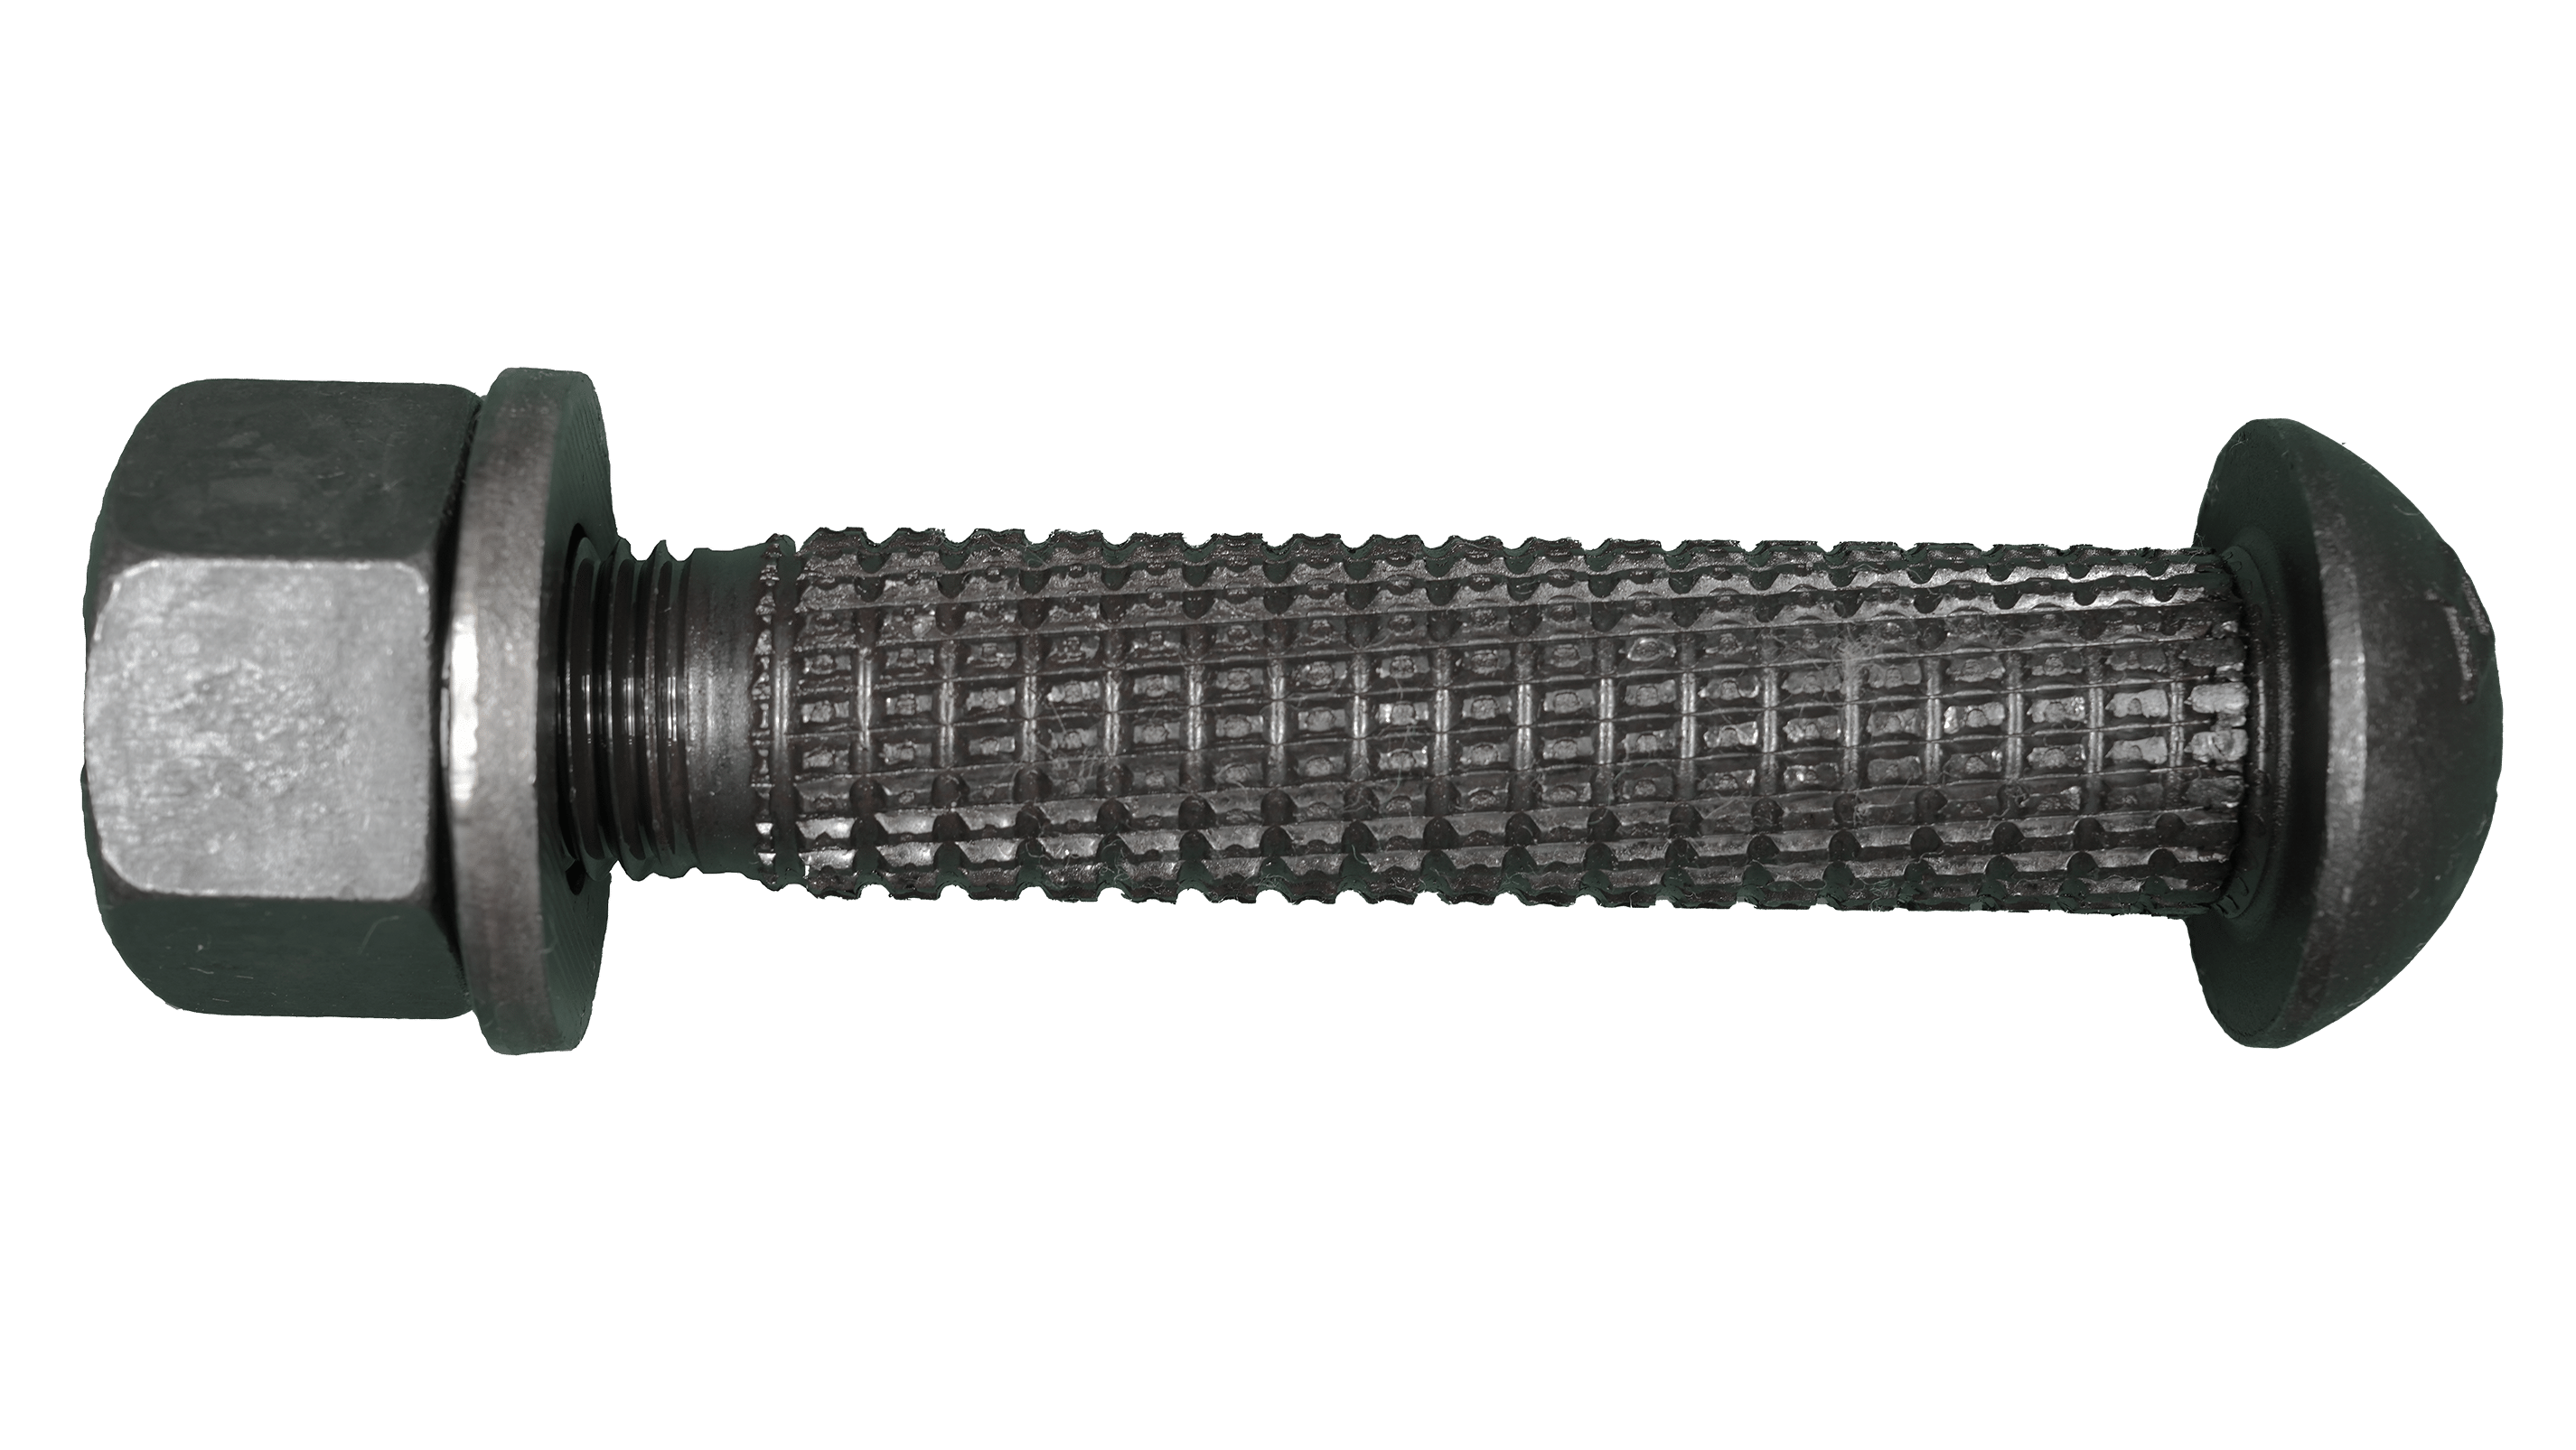
\includegraphics[width=0.5\textwidth]{imgs/ch6/oneBbolt.png}
    \caption{Interference fit bolt for Bearing-type connection (M22, Diameter = 23.5mm, Courtesy of Kobelco Bolt, Ltd.)}
    \label{ch6fig-onebbolt}
\end{figure}

For bearing-type bolted connections, AASHTO LRFD BDS 2020 \cite{AASHTO2020} defines it as a strength limit state only for joints subjected to axial compression or joints on bracing members. Both Eurocode3 EN 1993-1-8:2021 \cite{eurocode3-21}and GB50017-2017 \cite{gb50017-2017}define that it should be designed in the same way as friction-type bolted connections, and define the serviceability limit state as slip resistance and the bearing resistance as the ultimate limit state. However, Eurocode 3 allows the bearing resistance of resin and slip resistance of injection bolts to be accumulated for design under the serviceability limit state, and Japanese's JSHB-2017 \cite{douji2017} states that bearing type bolted connections could be designed to meet serviceability limit state by bearing resistance. 


\section{Experiment}

\subsection{Material test}

The material test specimens were prepared in accordance with JIS Z 2241 2011\cite{JIStest}. Material tests were conducted on three steel specimens of 50 mm and 28 mm thickness, respectively. The summary results are shown in Table \ref{tab-mtresult}. Plan view after material test as shown in Fig. \ref{fig-mt-1}. \par

and the load-strain relationships for the 50 mm thickness specimens are shown in Fig. \ref{fig-mt50-ls}

\begin{figure}[htbp]
    \centering
    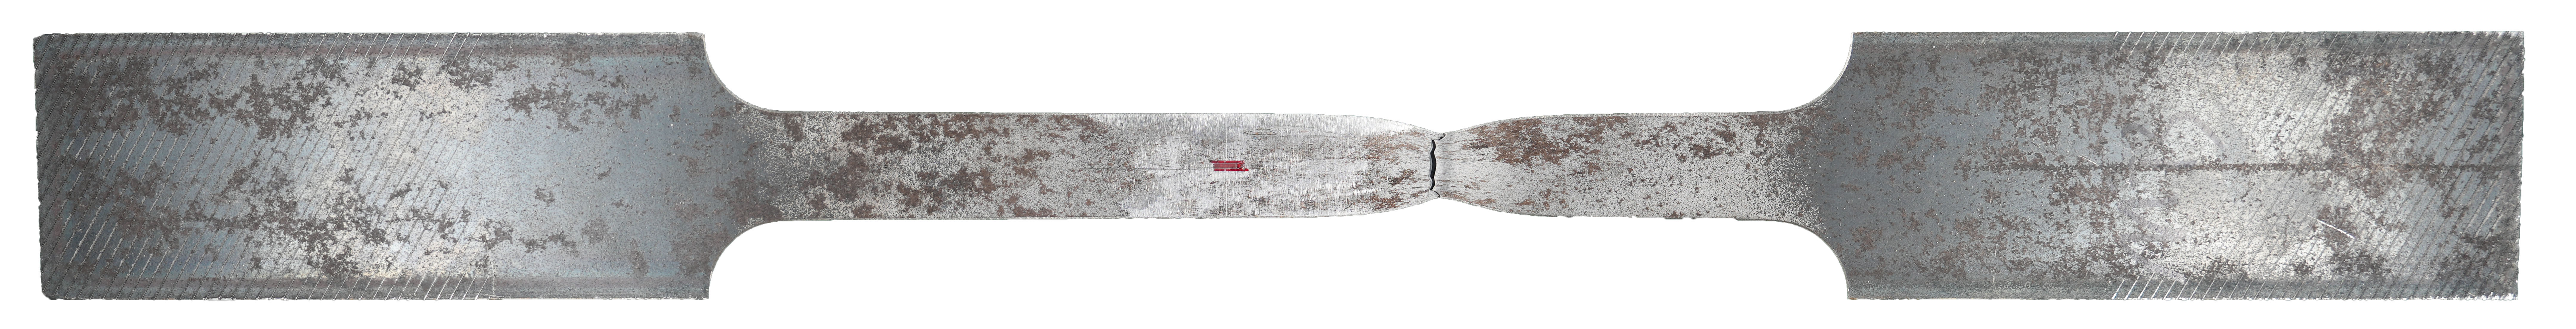
\includegraphics[width=0.8\textwidth]{imgs/ch6/mt-1.jpg}
    \caption{Plan view after material test}
    \label{fig-mt-1}
\end{figure}

\begin{figure}[htbp]
    \centering
    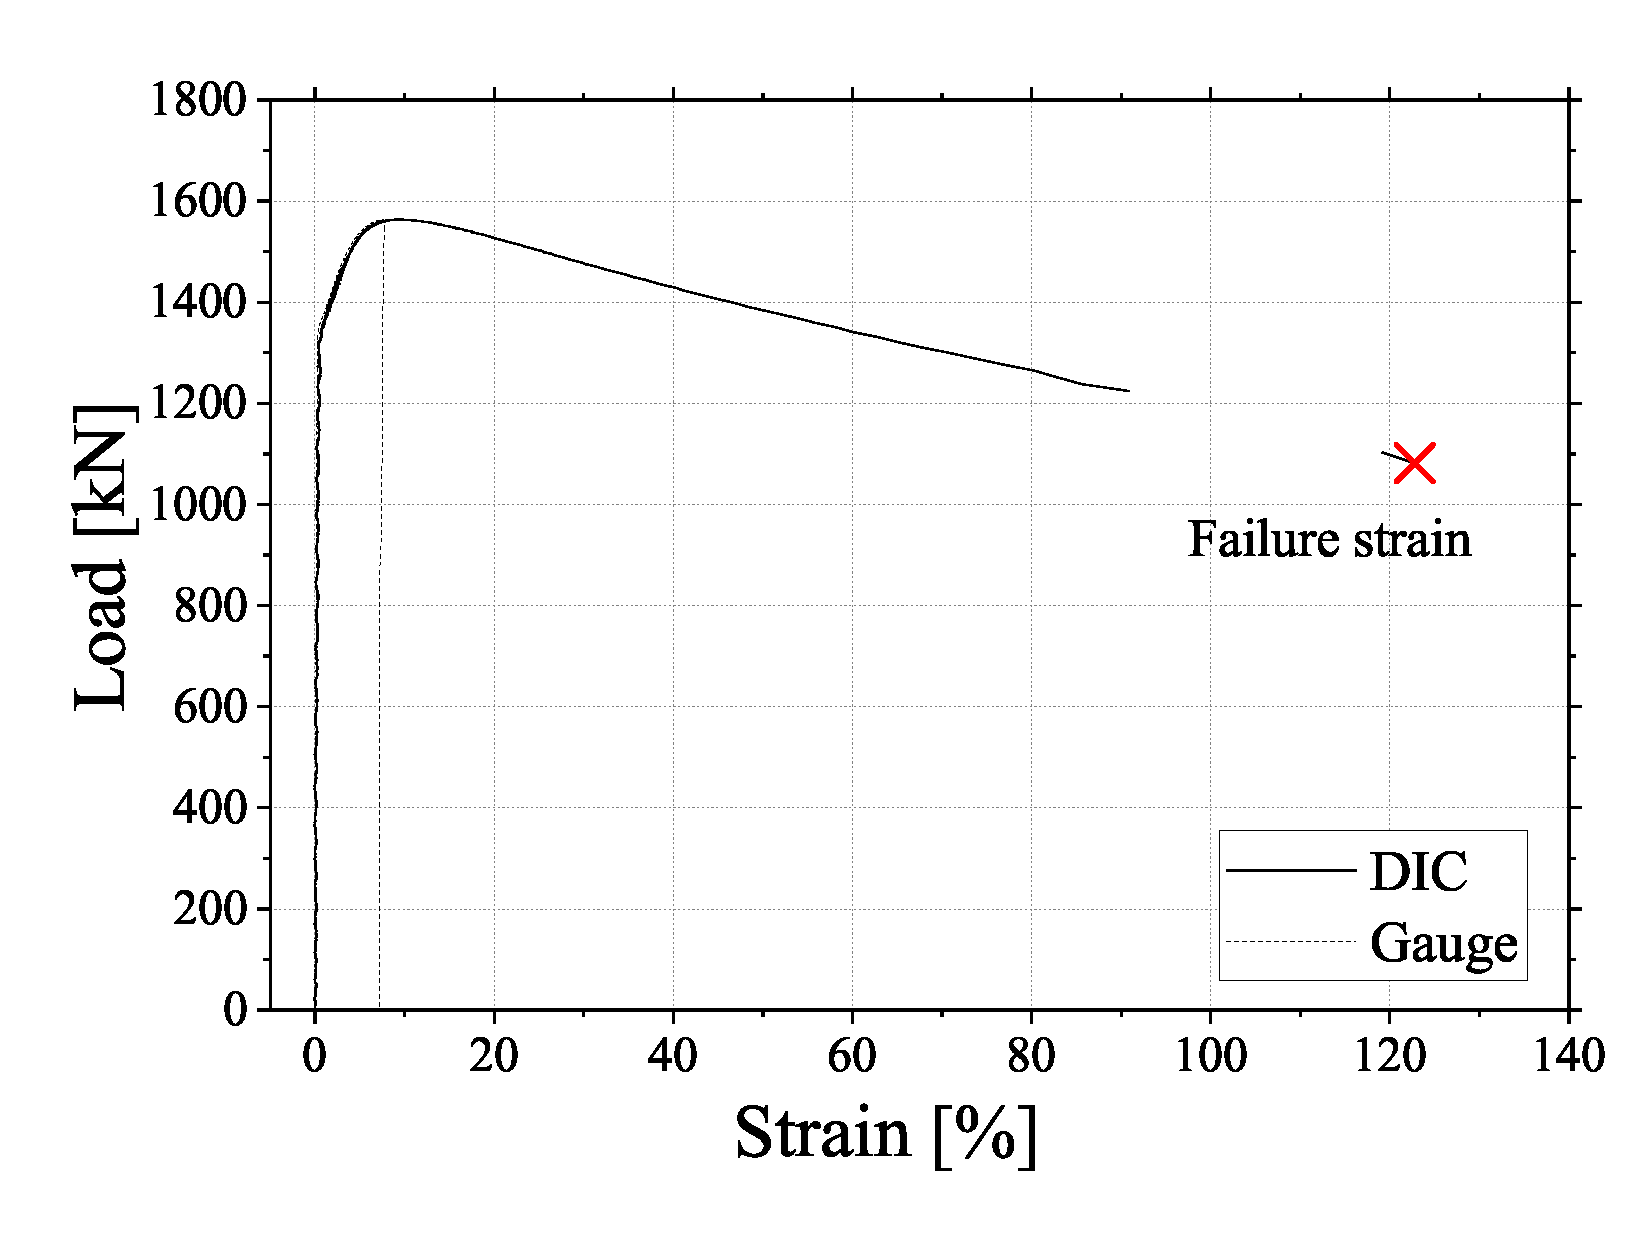
\includegraphics[width=0.6\textwidth]{imgs/ch6/mt50-LS.eps}
    \caption{The relationship between Load and Strain}
    \label{fig-mt50-ls}
\end{figure}

\begin{table}[htbp]
\centering
\caption{Material test results}
\label{tab-mtresult}
\begin{tabular}{@{}ccccccc@{}}
\toprule
\multirow{2}{*}{\begin{tabular}[c]{@{}c@{}}Component\\ name\end{tabular}} & \multicolumn{2}{c}{\begin{tabular}[c]{@{}c@{}}Plate\\ 28 mm \end{tabular}} & \multicolumn{2}{c}{\begin{tabular}[c]{@{}c@{}}Plate\\50 mm\end{tabular}} & \begin{tabular}[c]{@{}c@{}}Interference fit \\ bolt (B10T)\end{tabular} & \begin{tabular}[c]{@{}c@{}}High-strength \\ bolt (F10T)\end{tabular} \\ \cmidrule(l){2-7} 

& \begin{tabular}[c]{@{}c@{}}Inspection \\ Certificate\end{tabular} & \begin{tabular}[c]{@{}c@{}}Tensile \\ test\end{tabular} & \begin{tabular}[c]{@{}c@{}}Inspection \\ Certificate\end{tabular} & \begin{tabular}[c]{@{}c@{}}Tensile \\ test\end{tabular} & \multicolumn{2}{c}{\begin{tabular}[c]{@{}c@{}}Inspection \\ Certificate\end{tabular}} \\ \midrule

\begin{tabular}[c]{@{}c@{}}Yield Strength\\ {[}$N/mm^2${]}\end{tabular} & 536 & 525.5 & 549 & 548.6 & 1025 & 998 \\
\begin{tabular}[c]{@{}c@{}}Ultimate Strength\\ {[}$N/mm^2${]}\end{tabular} & 633 & 619.5 & 646 & 635.5 & 1073 & 1075 \\
\begin{tabular}[c]{@{}c@{}}Young's modulus $E$\\ {[}$KN/mm^2${]}\end{tabular} & - & 209 & - & 213 & - & - \\
Poisson's ratio $v$ & - & 0.274 & - & 0.269 & - &- \\
\begin{tabular}[c]{@{}c@{}}Elongation\\ {[}$\%${]}\end{tabular} & 26 & - & 46 & - & 19& 19\\ \bottomrule
\end{tabular}
\end{table}

\subsection{Standard slip test for measurement the slip coefficient}

The geometry of the standard slip test specimen is shown in Fig. \ref{fig-sliptest}, and the structural characteristics are shown in Table \ref{tab-sizeslip}. The geometry was prepared with reference to the high-strength bolt design, construction, and maintenance guidelines \cite{shishin2009}.

\begin{figure}[htbp]
    \centering
    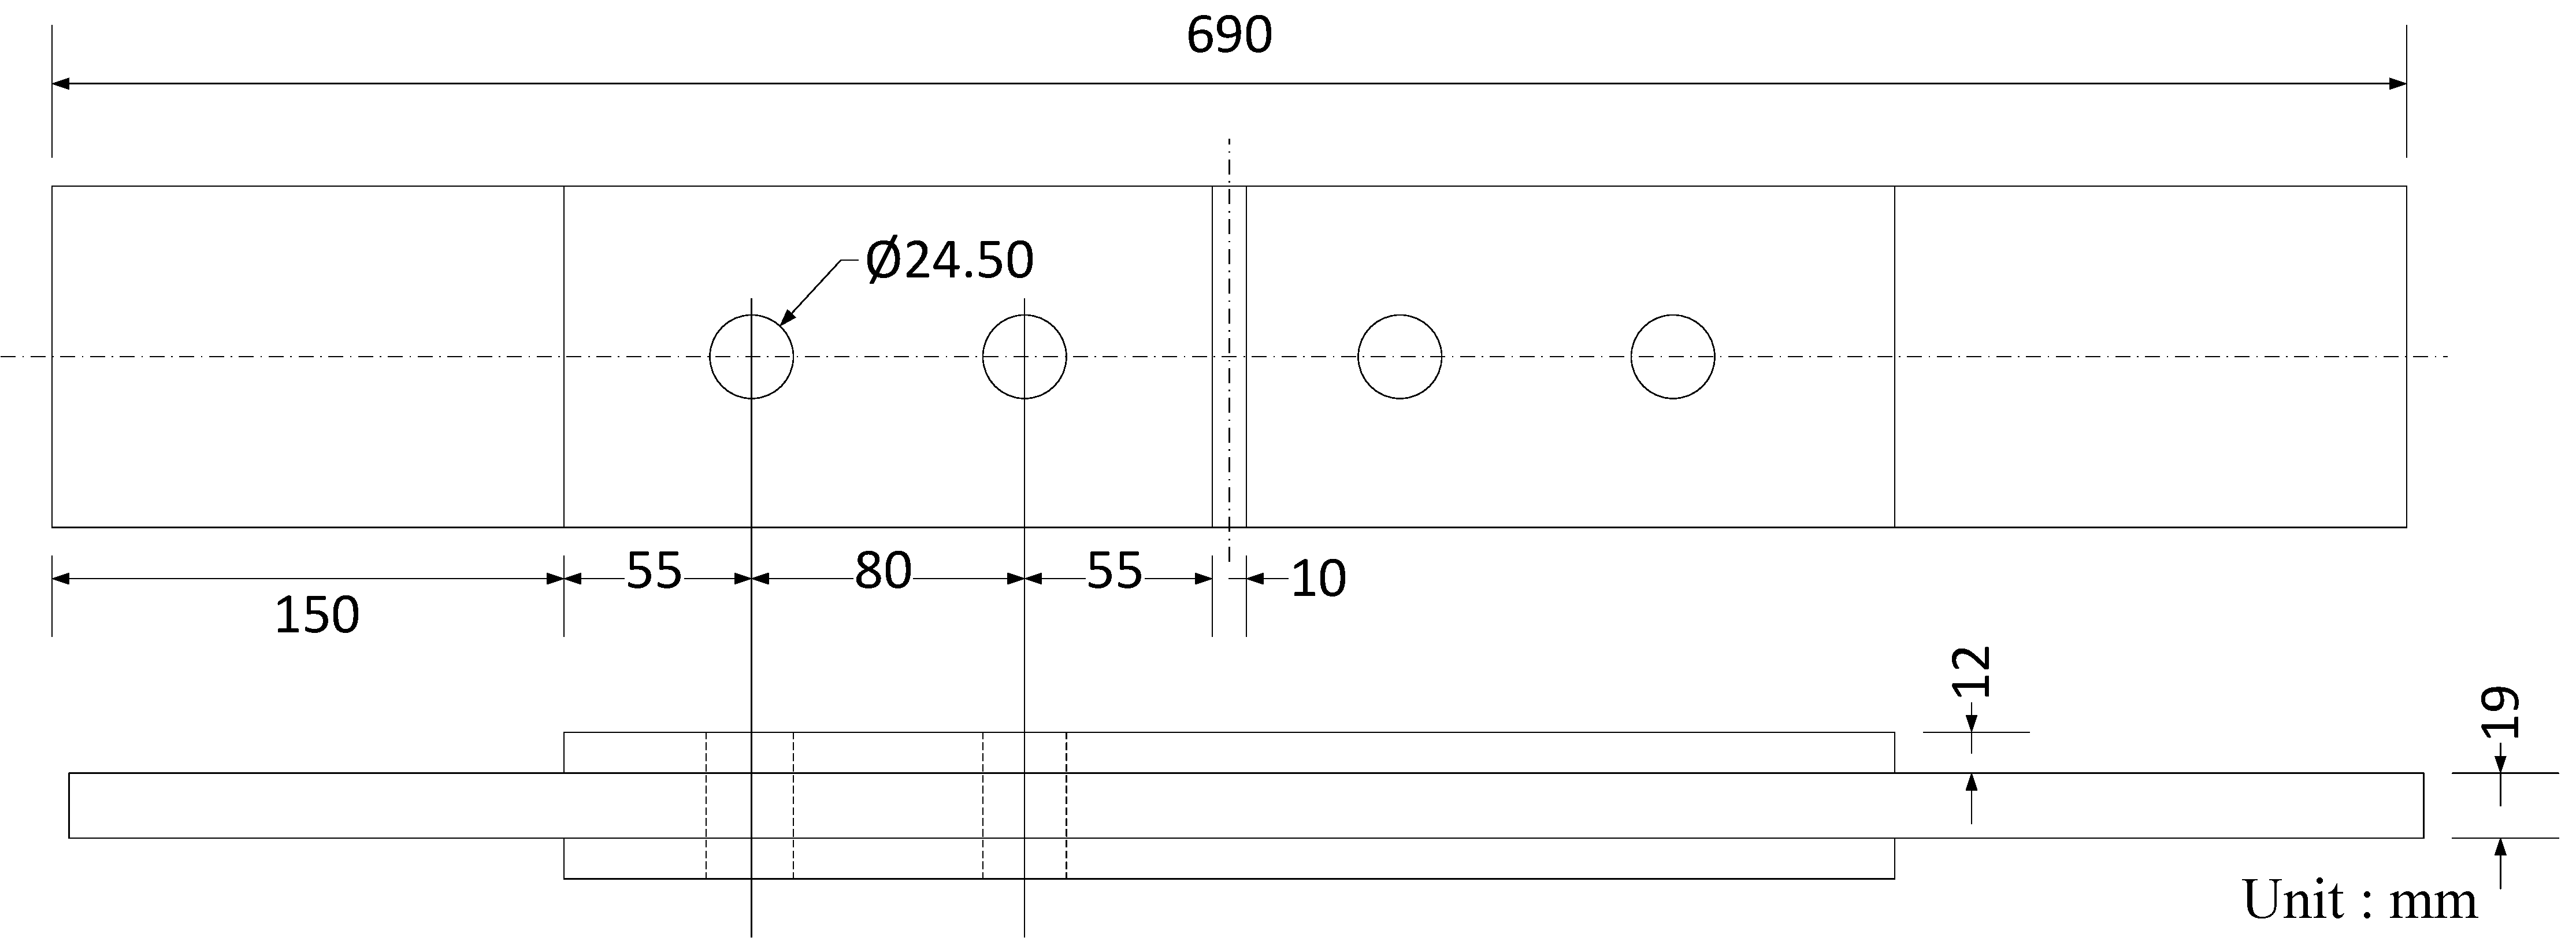
\includegraphics[width=0.85\linewidth]{imgs/ch6/slip-test.pdf}
    \caption{Shape of standard slip specimen}
    \label{fig-sliptest}
\end{figure}

\begin{table}[htbp]
\centering
\caption{Shape of standard slip specimen}
\label{tab-sizeslip}
\begin{tabular}{@{}cccccccccc@{}}
\toprule
 \begin{tabular}[c]{@{}c@{}}Bolt \\ grade\end{tabular}&
  \begin{tabular}[c]{@{}c@{}}$d$\end{tabular} &
  \begin{tabular}[c]{@{}c@{}}$d_0$\end{tabular} &
  \begin{tabular}[c]{@{}c@{}}Steel grade\end{tabular} &
  \begin{tabular}[c]{@{}c@{}}$f_y$\end{tabular} &
  \begin{tabular}[c]{@{}c@{}} $t_m$\end{tabular} &
  \begin{tabular}[c]{@{}c@{}}$t_s$\end{tabular} &
  \begin{tabular}[c]{@{}c@{}} $w$\end{tabular} &
  \begin{tabular}[c]{@{}c@{}}$e_1$\end{tabular} &
  \begin{tabular}[c]{@{}c@{}}$p_1$\end{tabular} 
  \\ \midrule
F10T & 22 & 24.5 & SM490Y & 355 & 19 & 12 & 100 & 55 & 80
\\ \bottomrule
\end{tabular}
\end{table}

where, $t_m$ is the thickness of main plate, $t_s$ is the thickness of splice plate, $w$ is the width of mian plate, $e_1$ is the end distance from bolt hole, $p_1$ is the bolt spacing. 

The test method for the standard slip test is shown below.

\begin{enumerate}
    \item The number of specimens shall be three. One side of the specimen is the test side and the other side is the fixed side. The bolts on the fixing side should be retightened by $10\%$ to prevent slippage at the test end. \\
    The slip coefficient $\mu$ is calculated by the following equation.
    \begin{equation}
    \mu = \frac{P}{m\times n \times N}
    \end{equation}
    where $P$: slip load measured by slip test, $m$: number of joint faces (=2), $m$: number of bolts (=2), $N$: design bolt axial force
    
    \item The joint surface treatment shall be the same as that of the adopted joint.
    In the 
    \item test, tensile loading is performed while measuring the relative displacement between the main plate and splice plate, and if no clear slip occurs, the measured relative displacement is used to determine the slip load (here, the relative displacement is used to determine the slip load). (In this case, slip is determined when the relative displacement reaches 0.2 mm.)
    \item The axial force introduced into the bolt is based on the standard axial force, and the test is conducted at least 12 hours after the bolt has been tightened, taking into account the effect of relaxation.
\end{enumerate}

The result of slip coefficient test as shown in table \ref{tab-slipcoef}, both the bolt preload and the slip coefficient have a low variation.

\begin{table}[htbp]
\centering
\caption{Result of slip coefficient test}\label{tab-slipcoef}
\begin{tabular}{@{}ccccc@{}}
\toprule
\multirow{2}{*}{Name} & \multicolumn{2}{c}{Preload} & \multirow{2}{*}{Slip load} & \multirow{2}{*}{Slip Coefficient} \\ \cmidrule(lr){2-3}
 & Before loading & Avg. &  &  \\ \midrule
\multirow{2}{*}{test-1} & 108.58 & \multirow{2}{*}{105.6} & \multirow{2}{*}{332.2} & \multirow{2}{*}{0.786} \\
 & 102.74 &  &  &  \\
\multirow{2}{*}{test-2} & 107.18 & \multirow{2}{*}{107.6} & \multirow{2}{*}{352.4} & \multirow{2}{*}{0.819} \\
 & 108.42 &  &  &  \\
\multirow{2}{*}{test-3} & 107.18 & \multirow{2}{*}{107.8} & \multirow{2}{*}{348.4} & \multirow{2}{*}{0.808} \\
 & 108.42 &  &  &  \\
Mean &  &  &  & 0.804 \\
Standard Deviation &  &  &  & 0.017 \\ \bottomrule
\end{tabular}
\end{table}


\subsection{Experiment detail}

The experimental specimen dimensions shown in Fig. \ref{fig-dimens} were selected based on previous research\cite{KAMEI2000} on the investigation results of an actual bridge. The commonly occurring single-row 10-column arrangement was used as a reference. To investigate the mechanical behavior of slip and bearing of the joints, $\beta$ is set to 0.65 to prevent the joints from being affected by the cross-sectional yield of the main plate before slip.

The specimens were subjected to loading using a hydraulic universal testing machine with a capacity of 2000kN (provided by Tokyo Testing Machine Co. Ltd.). Considering the testing machine's loading capacity, the specimen was scaled down to a size of 16/22. Static uniaxial tension testing was conducted. The loading rate was set to 1 kN/s until either the test machine capacity was reached or failure occurred in the net cross section of plate or shear of the bolt. The loading device is depicted in Fig. \ref{fig-setup}.

Fig. \ref{fig-mealoc} shows the locations where the relative displacement, joint deformatioin, and strain are measured. Clip displacement gauges are used to measure relative displacement. Joint deformation is measured using an LVDT. Strain is measured using a strain gauge and a camera. Additionally, random patterns are applied to the side-2 of joint to capture the strain and displacement on the lateral side of the joint using \ac{DIC} method. Validation of \ac{DIC} methods as shown in Fig. \ref{fig-dicresult}.

\begin{figure}[htbp]
    \centering
    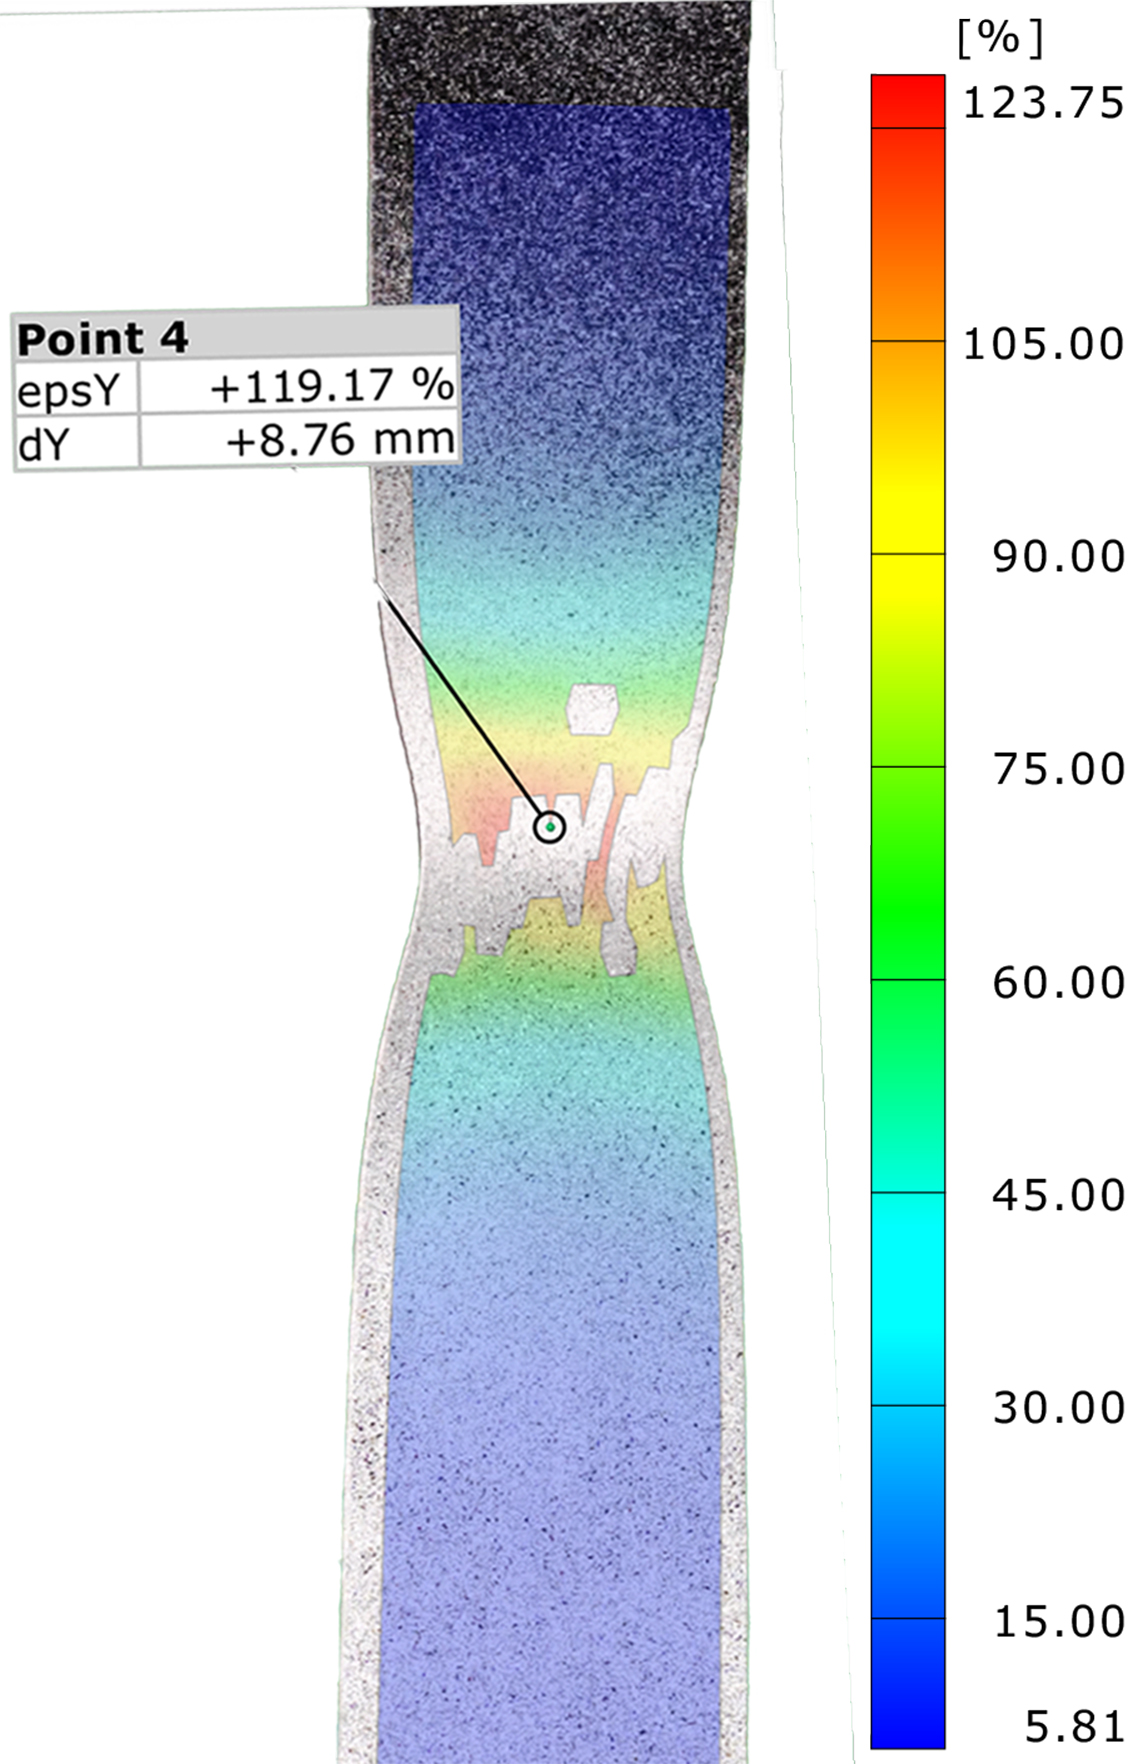
\includegraphics[width=0.4\textwidth]{imgs/ch6/DIC-RESULT.jpg}
    \caption{DIC-result}
    \label{fig-dicresult}
\end{figure}


According to JSHB\cite{douji2017}, the joint surface is coated with inorganic zinc-rich paint, with a presumed slip coefficient of 0.8, as determined from the slip factor test which arranged two bolts and have the same plate thickness and same faying surface condition as this test.

\begin{figure*}
    \centering
    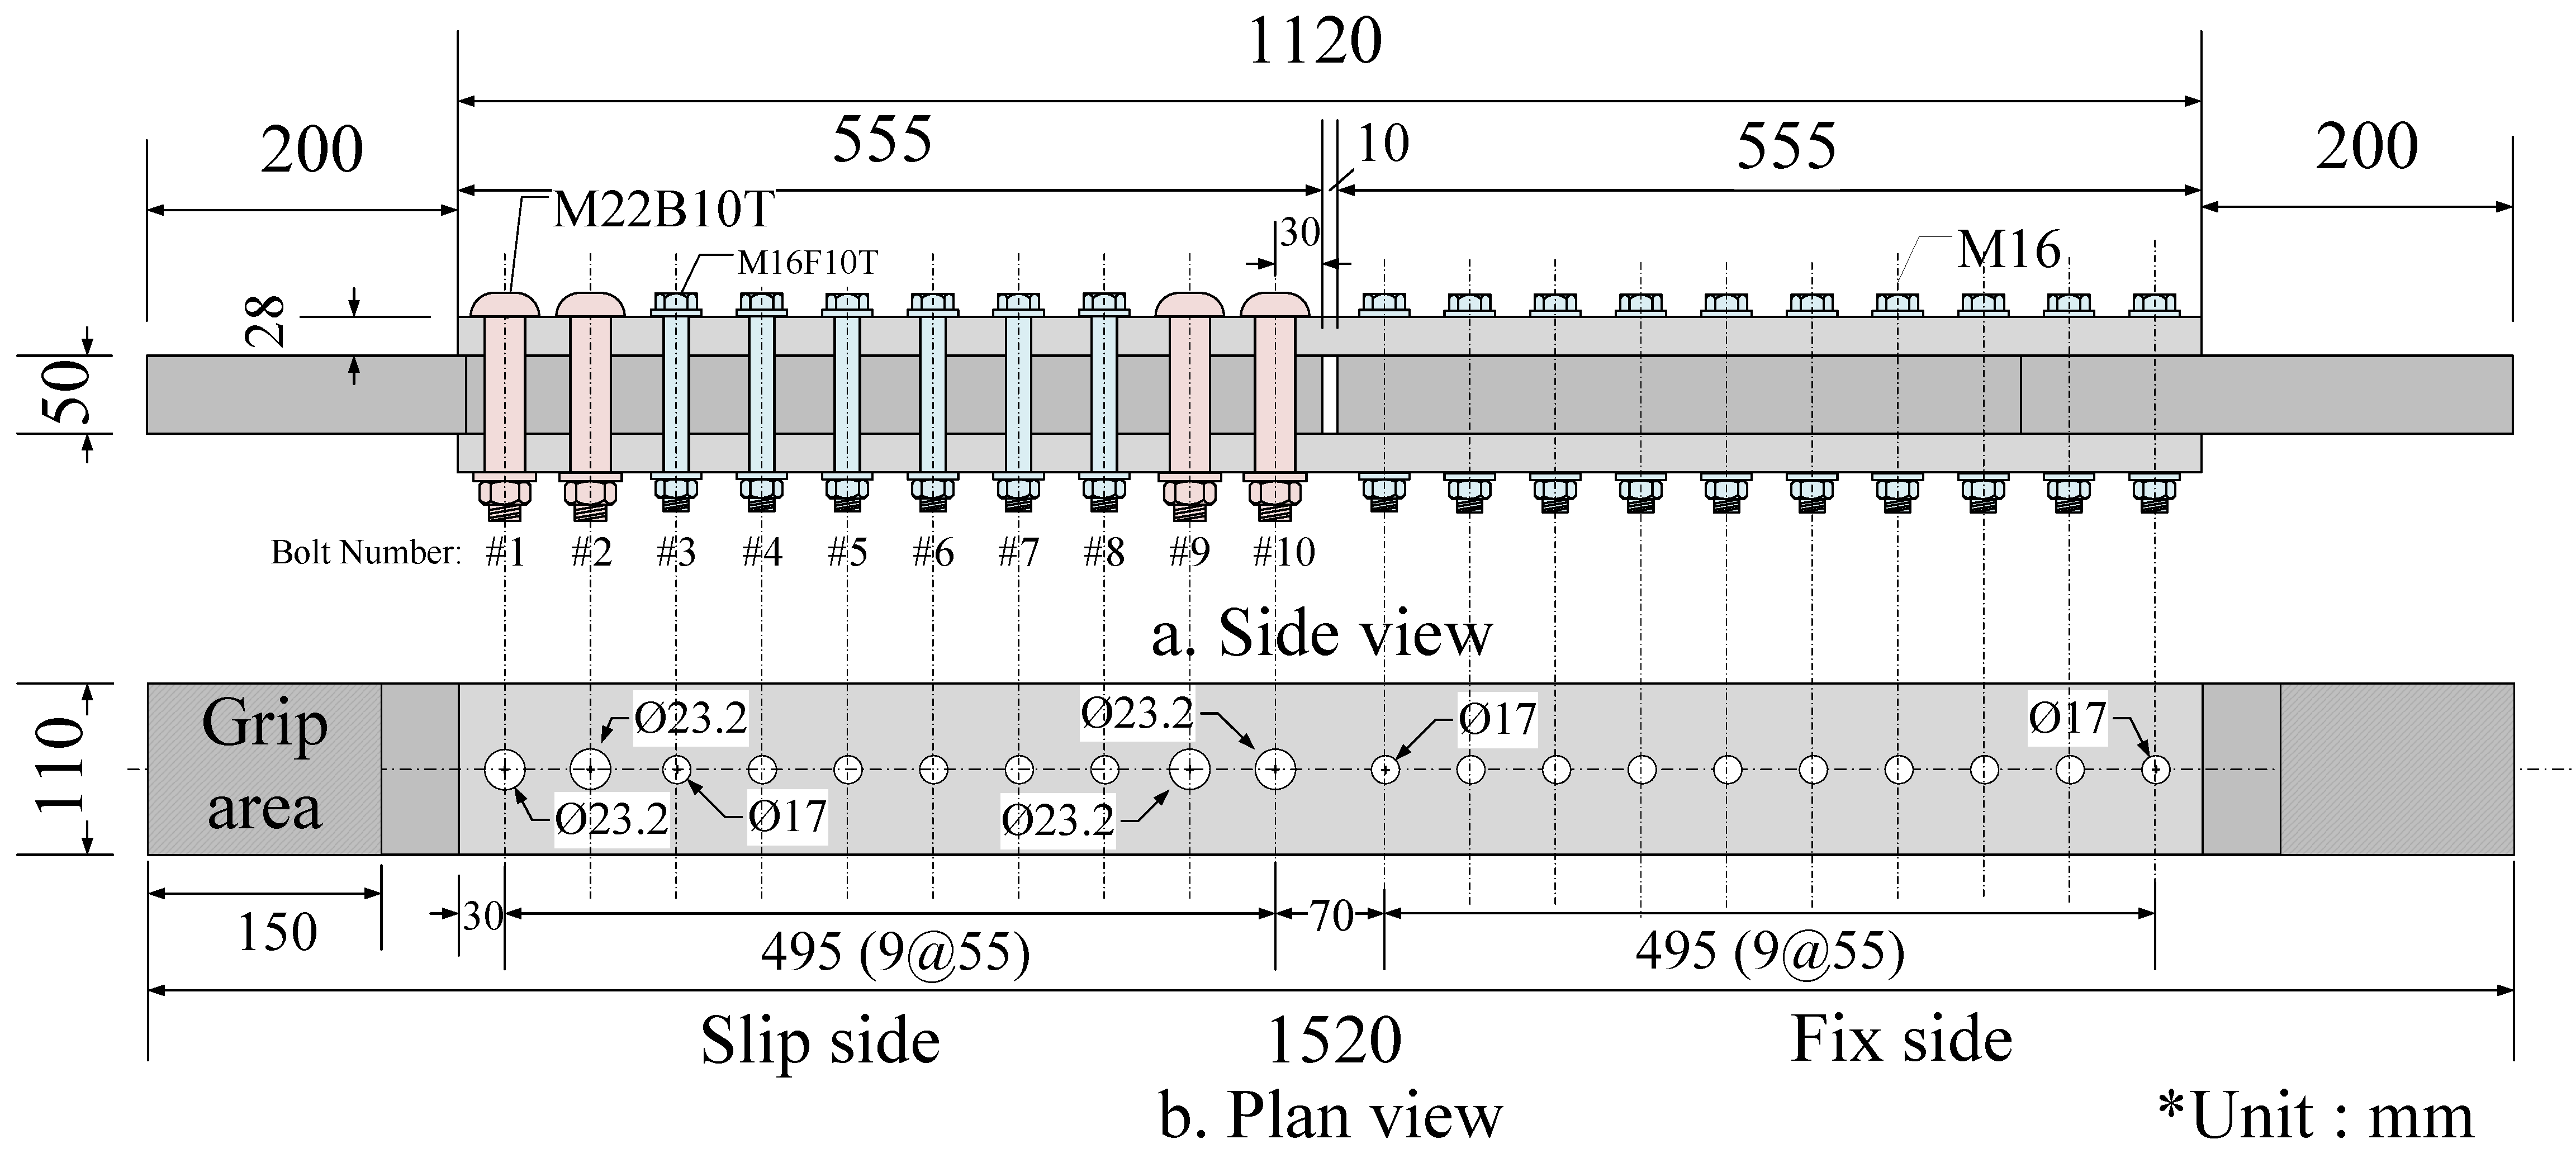
\includegraphics[width=\textwidth]{imgs/ch6/dimensions.pdf}
    \caption{Detailed dimensions of Hybrid joint}
    \label{fig-dimens}
\end{figure*}

\begin{figure}[htbp]
    \centering
    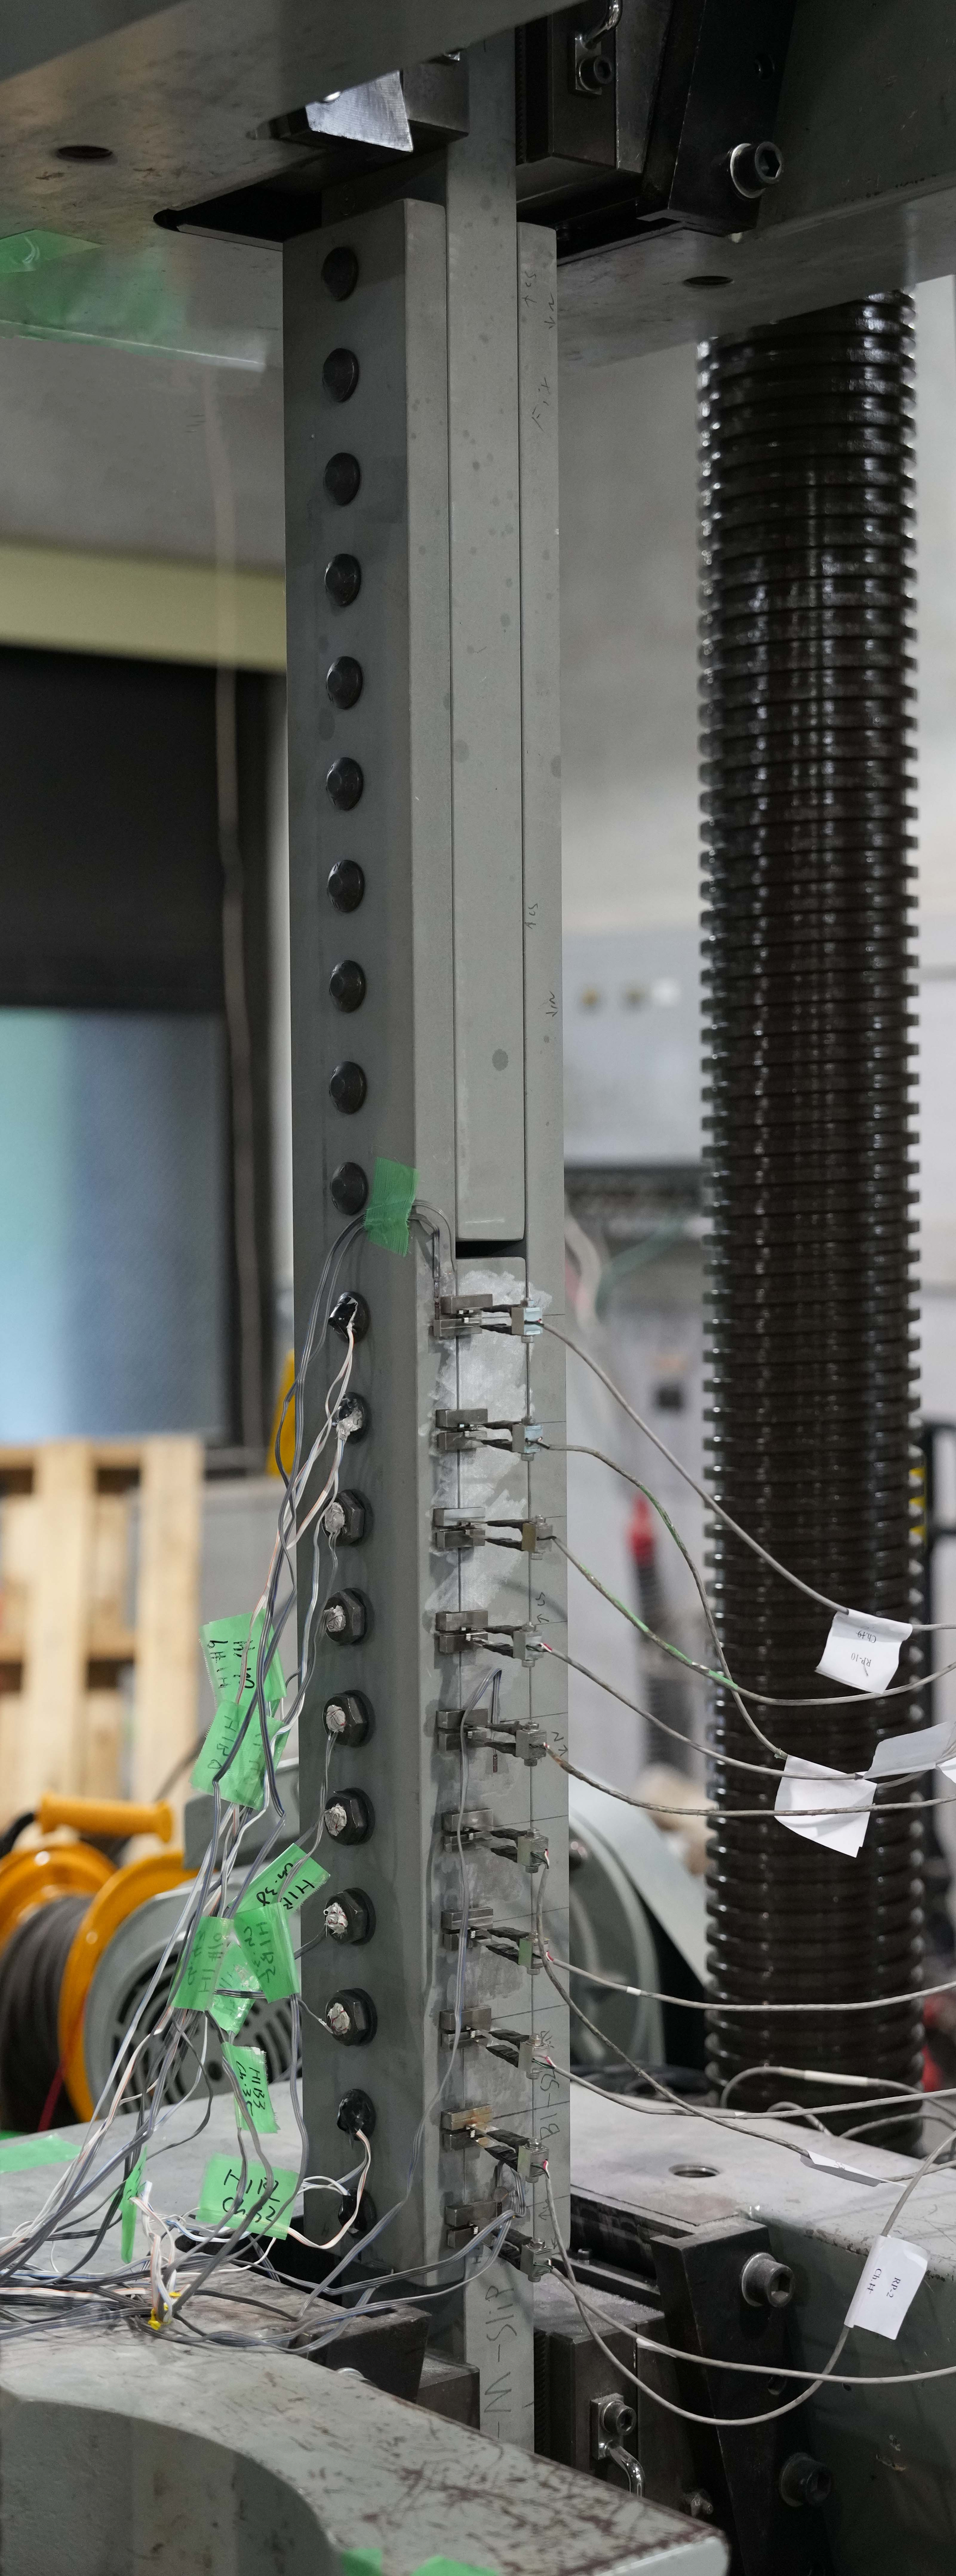
\includegraphics[width=0.25\textwidth]{imgs/ch6/set-up.jpg}
    \caption{Experiment Set-up}
    \label{fig-setup}
\end{figure}

\begin{figure*}
    \centering
    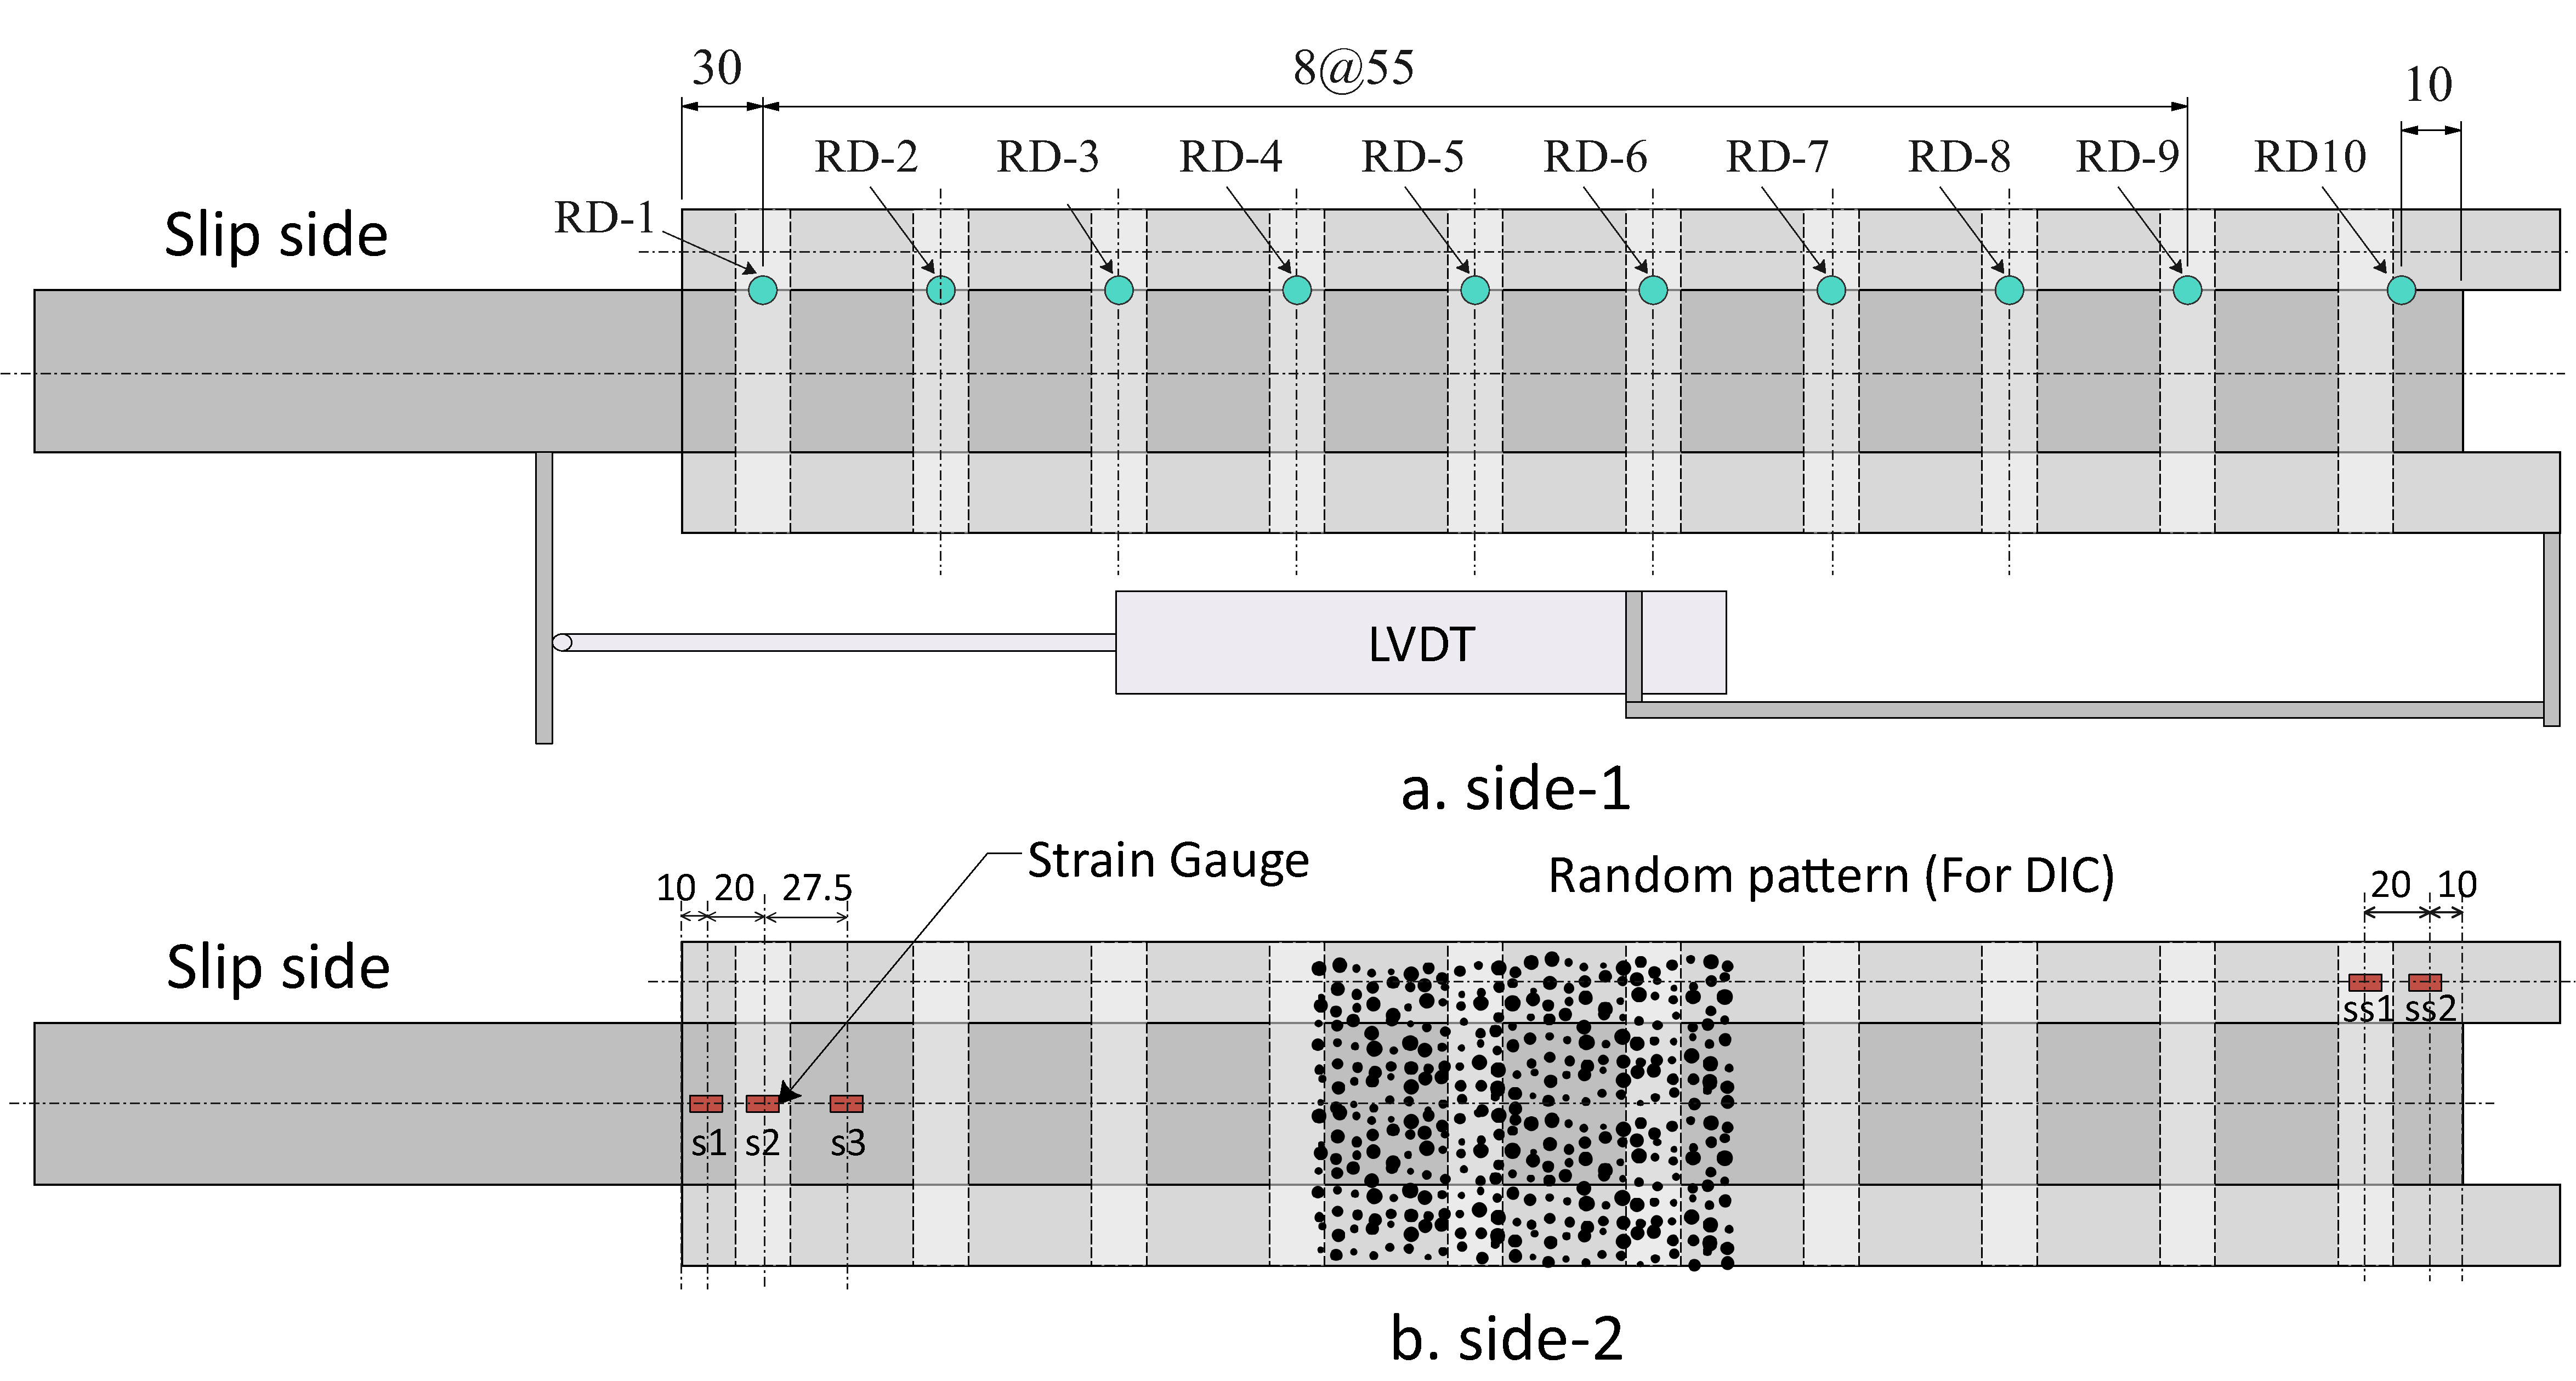
\includegraphics[width=0.9\textwidth]{imgs/ch6/mealoc.pdf}
    \caption{Measurement location (Unit: mm)}
    \label{fig-mealoc}
\end{figure*}

Interference fit bolts are installed using a hole with a diameter of 23.2mm. According to AASHTO \cite{AASHTO2020}, the common M16F10T bolt is installed using a 17mm diameter hole. Taking relaxation into account, the preload during installation for all bolts is 117kN \cite{douji2017}.

\subsection{Experimental cases}

The experimental specimens are shown in Table \ref{tab-expcase}. Previous research \cite{Chen2023MechanicalConnections} found that for long bolted joints with single columns of 8-12 rows, at least two or more Interference fit bolts should be used at each end of the joint to prevent excessive load sharing and premature shear yield of the bolts. Moreover, during the tightening process of the bolts, the bolt shank may undergo shrinkage caused by the Poisson's ratio effect, potentially leading to a loss of effectiveness in the interference fit. Therefore, in this experiment, the Hybrid case employs two Interference fit bolts at each end, whereas the Hybrid-NAF case means no preload for the interference fit bolt, which is only tightened to 5-10kN using a ratchet.

\begin{table*}[htbp]
\centering
\caption{ Experimental specimens }
\label{tab-expcase}
\begin{tabular}{@{}lcccccccccccc@{}}
\toprule
 \multirow{2}{*}{\begin{tabular}[c]{@{}c@{}} Specimens\end{tabular}} & \multicolumn{10}{c}{Fastener number (slip side)} & \multirow{2}{*}{\begin{tabular}[c]{@{}c@{}} Bolt \\ Preload\end{tabular}} \\ 
 \cmidrule(lr){2-11}
 &\multicolumn{1}{l}{\#1} & \multicolumn{1}{l}{\#2} & \multicolumn{1}{l}{\#3} & \multicolumn{1}{l}{\#4} & \multicolumn{1}{l}{\#5} & \multicolumn{1}{l}{\#6} & \multicolumn{1}{l}{\#7} & \multicolumn{1}{l}{\#8} & \multicolumn{1}{l}{\#9} & \multicolumn{1}{l}{\#10} &  \\ \midrule
Friction  &\faCircleO&\faCircleO&\faCircleO&\faCircleO&\faCircleO&\faCircleO&\faCircleO&\faCircleO&\faCircleO&\faCircleO& 117 \\
Hybrid & \faGear&\faGear&\faCircleO&\faCircleO&\faCircleO&\faCircleO&\faCircleO&\faCircleO&\faGear&\faGear& 117 \\
Hybrid-NAF & \faGear&\faGear&\faCircleO&\faCircleO&\faCircleO&\faCircleO&\faCircleO&\faCircleO&\faGear&\faGear& 5 --10 \\
\bottomrule
&&&&\multicolumn{9}{r}{\faCircleO : High-strength bolt, \faGear : Interference fit bolt}\\

\end{tabular}
\end{table*}


\section{Experiment Results}

\subsection{Installation of Interference fit bolt}
According to the regulations in Japan Road Association -- Japan Specifications For Highway Bridges - Part ii Steel Bridges\cite{douji2017} (hereinafter referred to as JSBH), the precision requirement for the bolt hole corresponding to the M22 bolt in bearing-type connections is 23.5±0.3mm. However, the maximum measured outer diameter of the Interference fit bolt shaft is 23.6mm. In order to confirm that the bolt can interference fit with the bolt hole after installation and fit tightly together, specimens with bolt hole diameters of 23.6mm, 23.5mm, and 23.2mm were respectively produced. Five interference fit bolts were randomly selected, and the average maximum  outer diameter of the bolt shaft (including the rib) measured with vernier calipers was 23.5 + 0.1mm.

The hole creation method involved drilling a pilot hole that is 1mm smaller than the target diameter, followed by enlarging the hole to the target diameter using a reamer. This approach guarantees that the bolt hole's accuracy is within ± 0.02mm.

The results showed that when the bolt hole is 23.6mm, the bolt can easily pass through the hole without achieving an interference fit. When the bolt hole is 23.5mm, it is not possible to insert the bolt into the hole by hand, but a hammer can be used with less force to install the bolt into the hole. When the bolt hole is 23.2mm, a significant amount of force is required to hammer the bolt into the hole.

Fig. \ref{fig-bcrossec} shows the cross-section of the bolt and the test plate. In both the 23.5mm and 23.2mm diameter holes, it can be observed that the ribs of the bolt have undergone plastic deformation, resulting in an interference fit. Fig. \ref{fig-bcrossec} reveals that the degree of deformation is more significant in the bolt shaft ribs and the hole wall of the test piece with the 23.2mm diameter hole. In order to achieve a better interference fit for the bolt, the diameter of the bolt hole for the Interference fit bolt used in this experiment was set to 23.2mm.


\begin{figure*}
\centering
\begin{subfigure}[t]{0.9\textwidth}
    \centering
    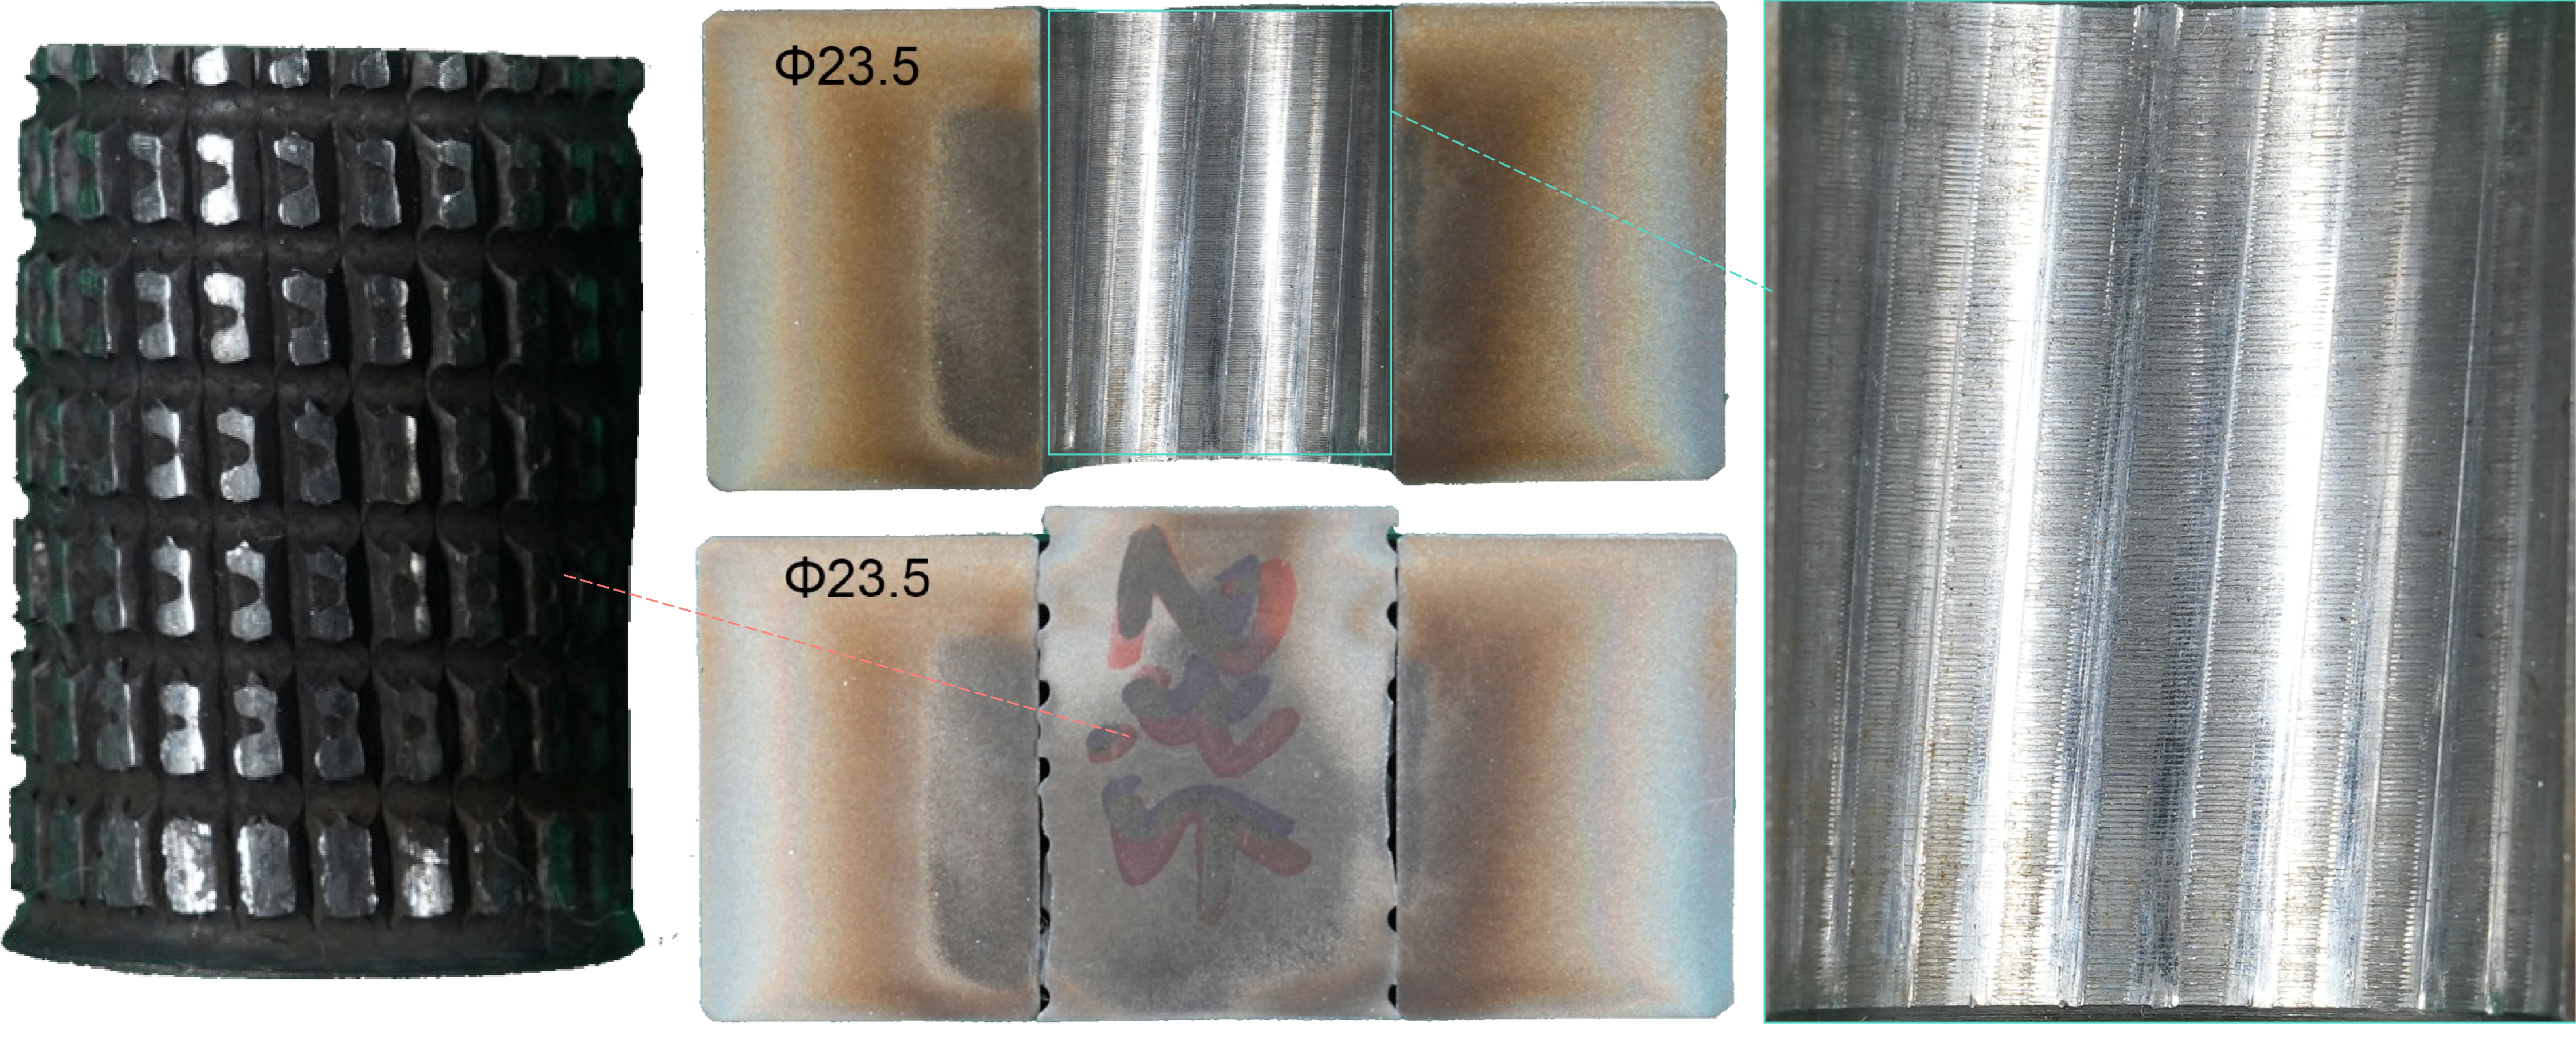
\includegraphics[width=\textwidth]{imgs/ch6/bstatus-23-5.pdf}
    \label{fig-bstatus235}
    \caption{23.5mm}
\end{subfigure}
\hfill
\begin{subfigure}[t]{0.9\textwidth}
    \centering
    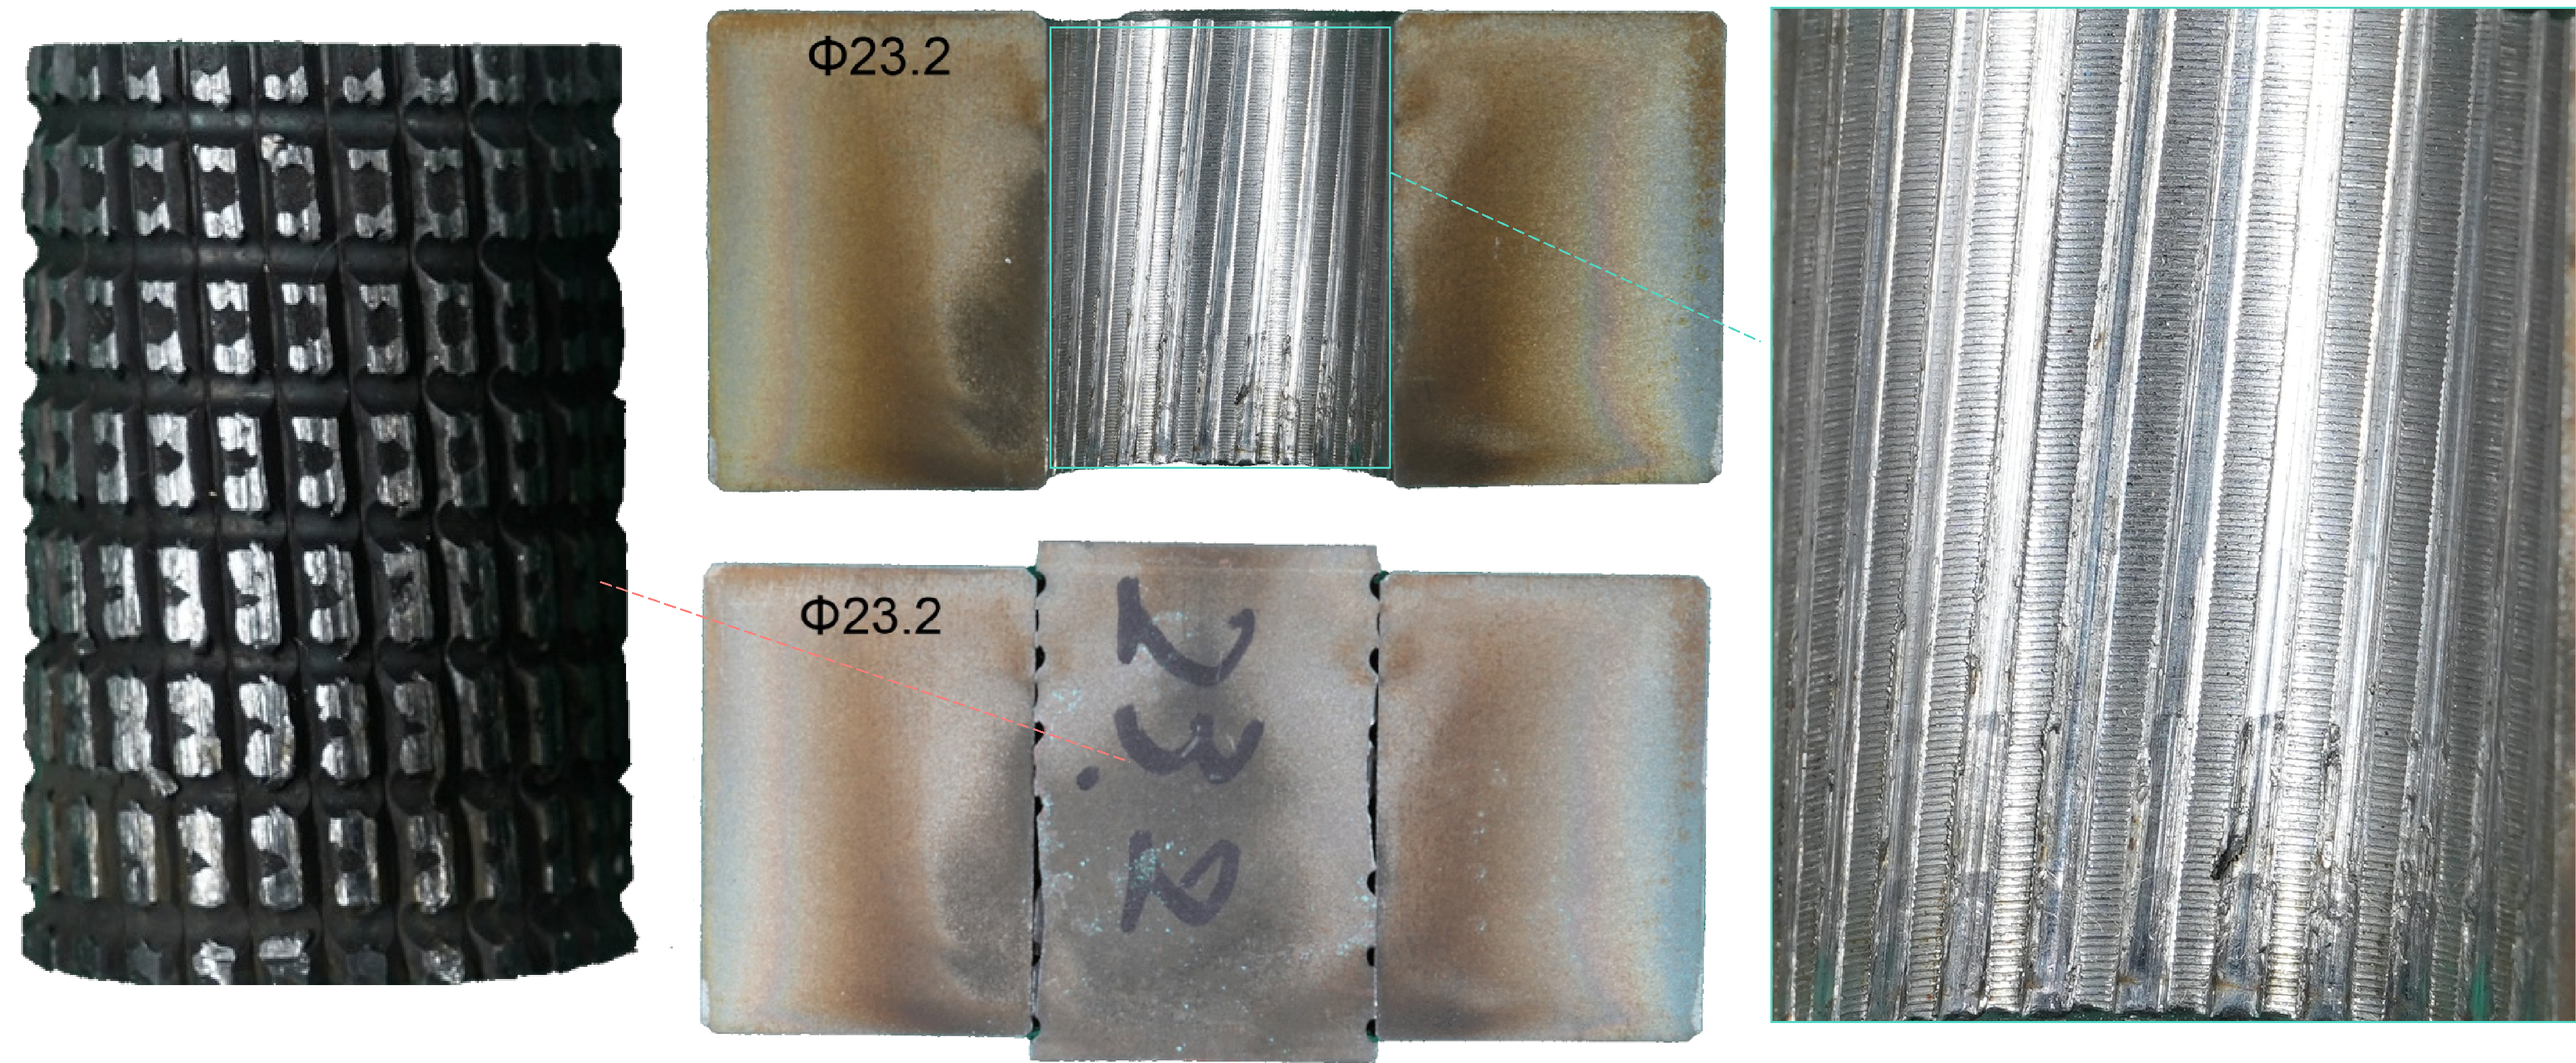
\includegraphics[width=\textwidth]{imgs/ch6/bstatus-23-2.pdf}
    \caption{23.2mm}
\end{subfigure}
\caption{The bearing status of the bolt shank and bolt hole.}
\label{fig-bcrossec}
\end{figure*}


\subsection{Deformation and relative displacement}

Fig. \ref{fig-loaddisp} shows the relationship between the load and the whole deformation of the joint. Clear slippage occurred at the friction type joint at 1361 kN, with the load decreasing to approximately 1048 kN (a change rate of approximately 23\%). The overall deformation of the joint increased from 3.7 mm to 6.5 mm, (a change rate of approximately 75\%). For the hybrid joint, slippage occurred when the load reached 1456 kN, and the load decreased from 1456 to 1407 kN (a change rate of approximately 3\%). As for the joint deformation, it decreased from 3.955 mm to 3.989 mm (a change rate of only approximately 0.8\%). The overall load-deformation relationship of the hybrid joint remains quasi-linear up to the upper load limit of 1800 kN, although a minor amount of slip occurs, and there have only 1mm minor residual deformation. In addition, for the Hybrid-NAF case, compare to the hybrid case besides a slight decrease in the initial slope and a minor reduction in the slippage load, the trend of the curve is not significantly different.

Fig. \ref{fig-rd10} shows the relationship between load and relative displacement at a distance of 10 mm from the end of main plate(CDT-6). Similar to the overall deformation figure, significant slippage occurred at the friction joint, with relative displacement increasing from 0.163 to 1.632 (an increase of approximately 900\%). As for the hybrid joint, the relative displacement increased from 0.184 to 0.342 (an increase of approximately 85\%). The hybrid joint exhibits a small amount of slippage similar to the results of previous studies\cite{kamei2010} on experiment of individual interference-fit bolts. This is due to the existence of small clearance between the bolt hole wall and the rib of the Interference fit bolt, resulting in inevitable slight slippage. The slip load of hybrid joints is 7\% higher than that of friction joint joints.

The value of slip load reduction and the slippage was summarized in Table \ref{tab-sumld}.

\begin{figure}[htbp]
\centering
    \begin{subfigure}[t]{0.45\textwidth}
        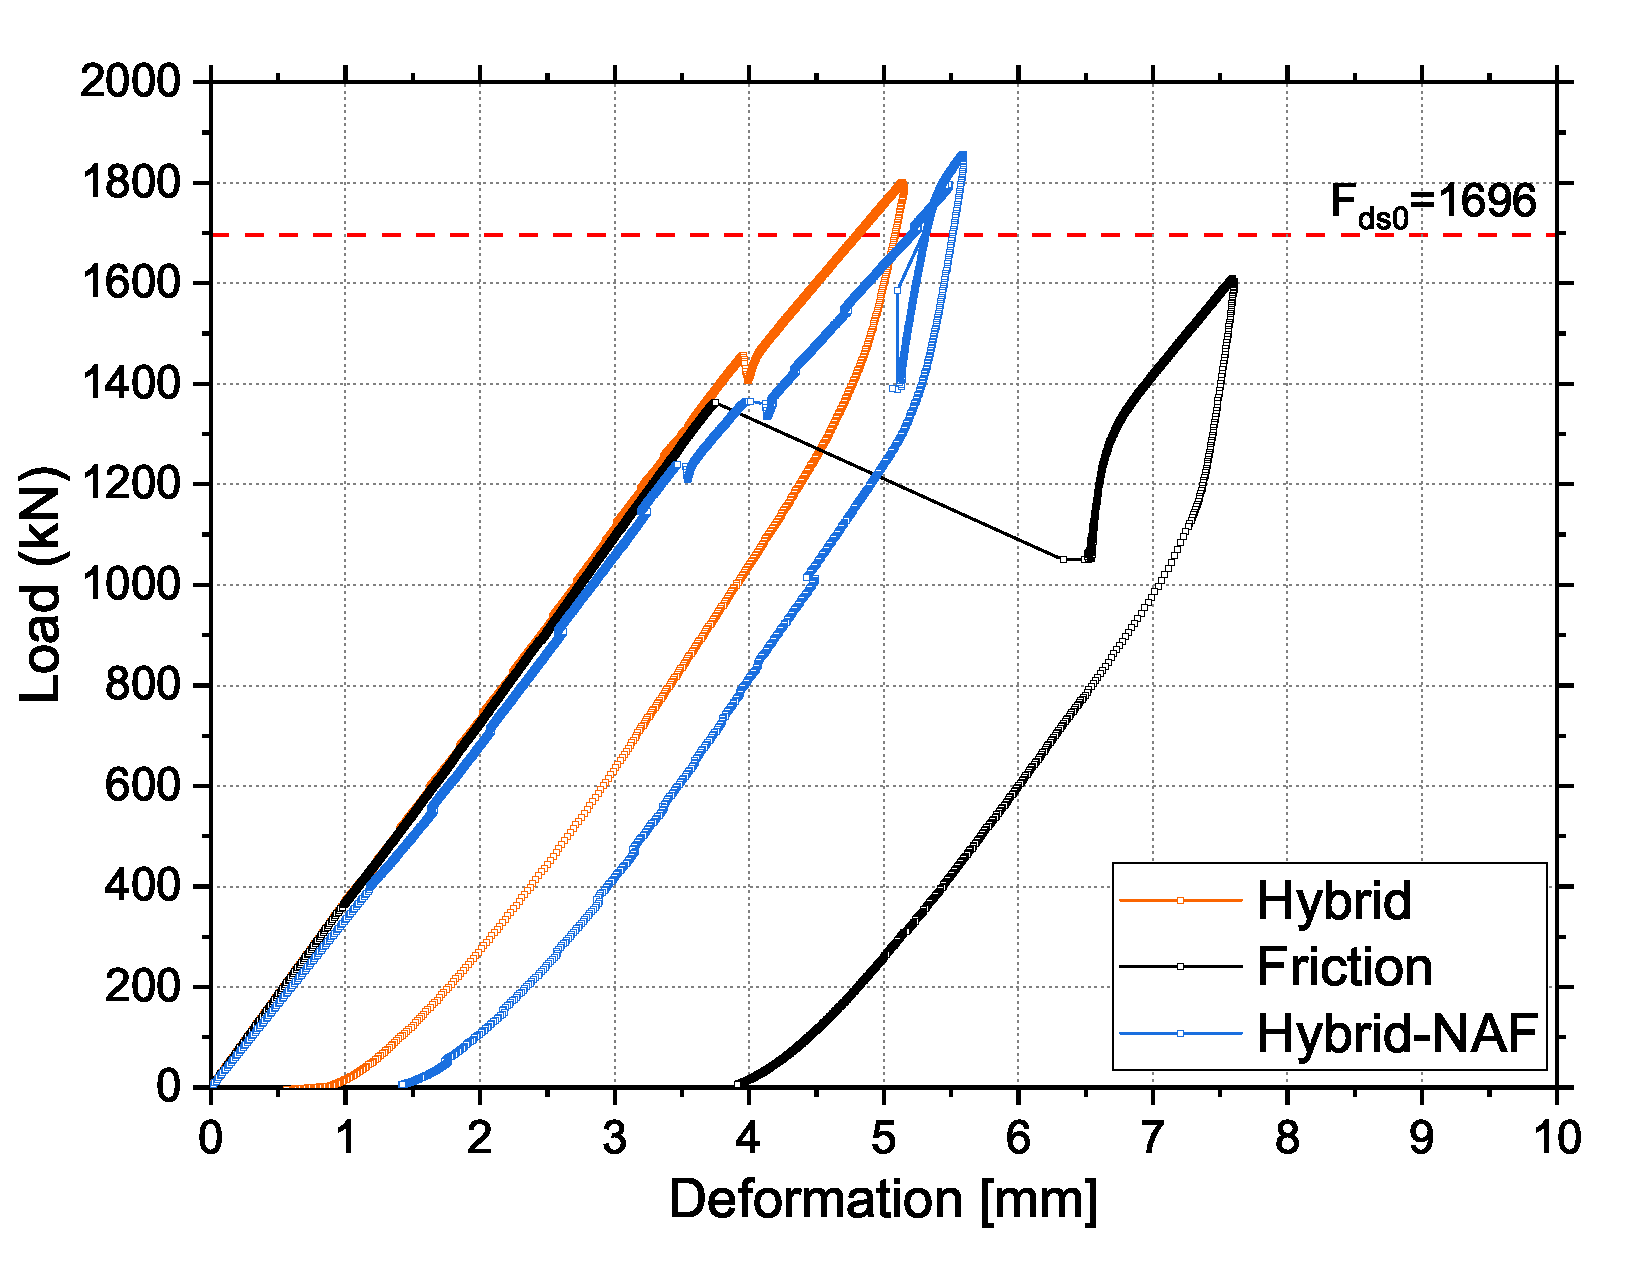
\includegraphics[width=\linewidth]{imgs/ch6/load-disp-cor.eps}
        \caption{Deformation}
        \label{fig-loaddisp}
    \end{subfigure}
    \hfill
    \begin{subfigure}[t]{0.45\textwidth}
        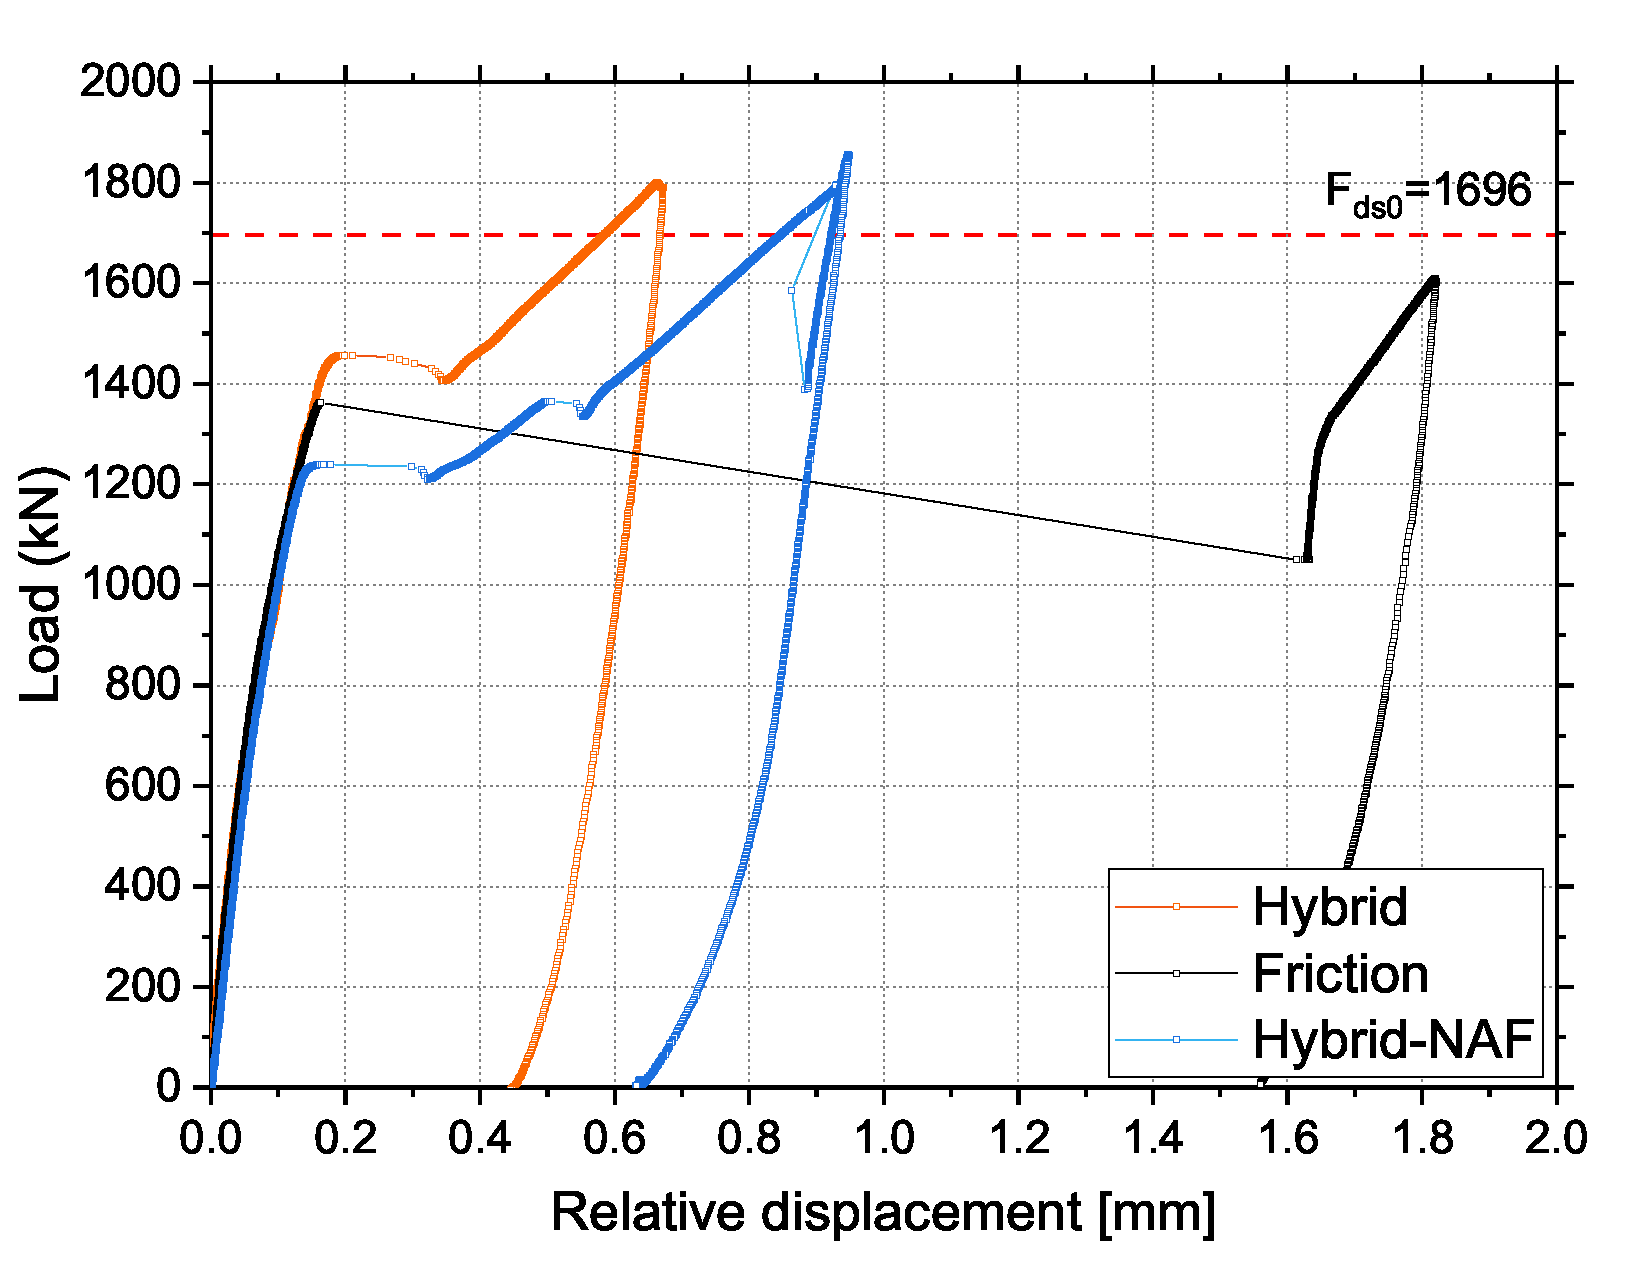
\includegraphics[width=\linewidth]{imgs/ch6/RD-bolt10.eps}
        \caption{Relative displacement}
        \label{fig-rd10}
    \end{subfigure}
    \caption{Relationship between load and deformation or relative displacement}
    \label{fig-disp}
\end{figure}


\begin{table}[]
\centering
\caption{ Summary of load drop and slip }
\label{tab-sumld}
\begin{tabular}{@{}ccccc@{}}
\toprule
Case & Slip Begins & End of Slip & Difference & Rate of Change \\ \midrule
\multicolumn{5}{c}{Load {[}kN{]}} \\
Friction & 1361 & 1048 & -313 & -23\% \\
Hybrid & 1456 & 1407 & -49 & -3\% \\
Hybrid-NAF & 1238 & 1210 & -28 & -2.2\% \\
\multicolumn{5}{c}{Deformation {[}mm{]}} \\
Friction & 3.7 & 6.5 & 2.8 & +75\% \\
Hybrid & 3.955 & 3.989 & 0.034 & +0.8\% \\
Hybrid-NAF & 3.46 & 3.54 & 0.08 & +2.3\% \\
\multicolumn{5}{c}{Relative Displacement {[}mm{]}} \\
Friction & 0.163 & 1.632 & 1.469 & +901\% \\
Hybrid & 0.184 & 0.342 & 0.158 & +85\% \\ 
Hybrid-NAF & 0.146 & 0.327 & 0.181 & +124\% \\ 
\bottomrule
\end{tabular}
\end{table}




\subsection{Bolt preload}

Fig. \ref{fig-laf} shows the relationship between bolt preload reduction ratio and load of each bolt, the bolt preload reduction ratio is calculated by $N/N_0$, where $N$ is real-time bolt preload, and $N_0$ is the bolt preload before loading. 

For the Friction joint, the most significant decrease in bolt preload occurred on bolt \#10, where the preload dropped to about 90\% when slip occurred (1361kN) as shown in Fig. \ref{fig-laff}. This is a 5\% difference compared to bolt \#6, which had the smallest decrease in preload.  The main reason for the significant reduction in preload at bolt \#10 is that the deformation of the splice plate at bolt \#10 is greater than that of the main plate at bolt \#1. Although the main plate had a larger net cross-sectional than the splice plate, considering the 1.1 times stress enhancement due to friction on the net cross-section of the main plate, the stress at the net cross-section of the splice plate would be almost the same as the main plate when subjected to the same tension. Moreover, it was found that the direct strain at bolt \# 10 of splice plate is greater than the strain at bolt \# 1 of main plate. Furthermore, apart from bolt \# 1, the preload of the other bolts have not decreased uniformly, with an approximate variation of 2\%. After 1361 kN was reached, a severe impact occurred due to the large slip that occurred in the joint and the momentary transition of the joint from a sliding to a bearing state, as a result, all strain gauges on the bolts were damaged and it was not possible to obtain bolt preload data.

For the hybrid joint as shown in Fig. \ref{fig-lafhy} , an observation was made that, at the load of 1361kN, there was a uniform distribution of bolt reduction ratio with a variation of around 1\% when compared to the friction type joint. Although we did not measure preload for the interference fit bolt, based on the data from HSB, we posit that the hybrid joint's load distribution is more uniform in comparison to the friction joint. Moreover, in the event that slip occurs at the joint, the variance of each bolt's preload is not significant, even after reaching 1456kN. When load reached 1800kN, the maximum reduction ratio in preload variation is only 6\%. Therefore, it can be considered that the load distribution of hybrid joints is more uniform and the load transmission is smoother than that of friction joints.

\begin{figure}[htbp]
    \centering
    \begin{subfigure}[t]{0.7\textwidth}
    \centering
    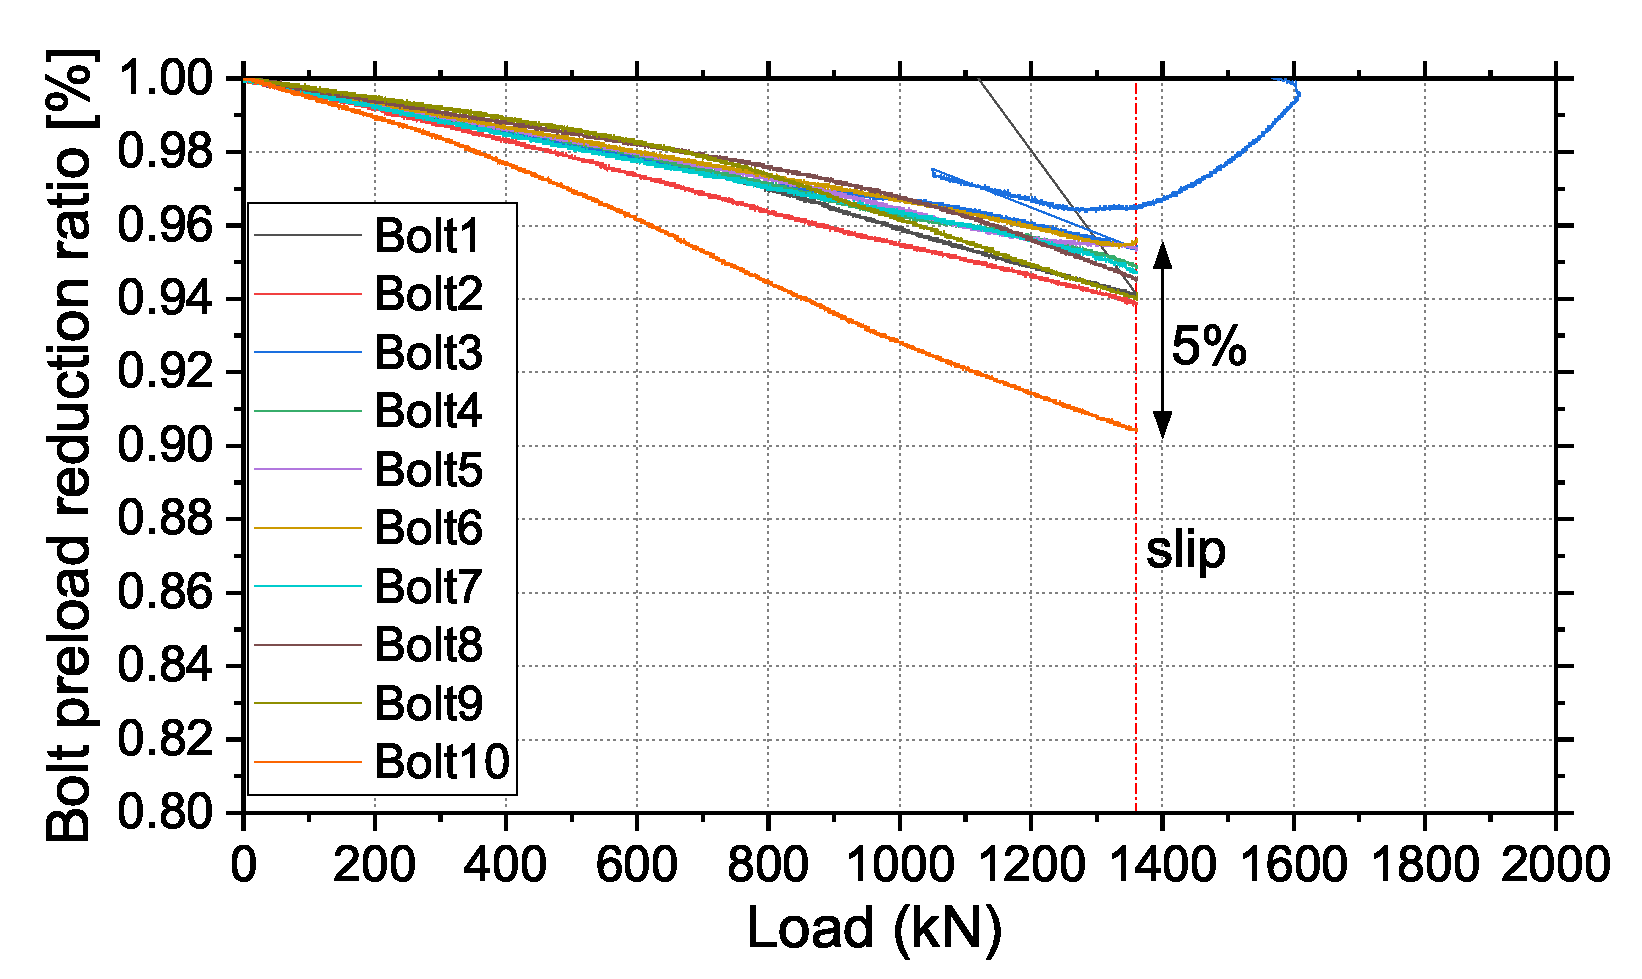
\includegraphics[width=\linewidth]{imgs/ch6/loadaf-fric.eps}
    \caption{Friction type joint }
    \label{fig-laff}
    \end{subfigure}
    %\vspace{1cm}
    \begin{subfigure}[t]{0.7\textwidth}
    \centering
    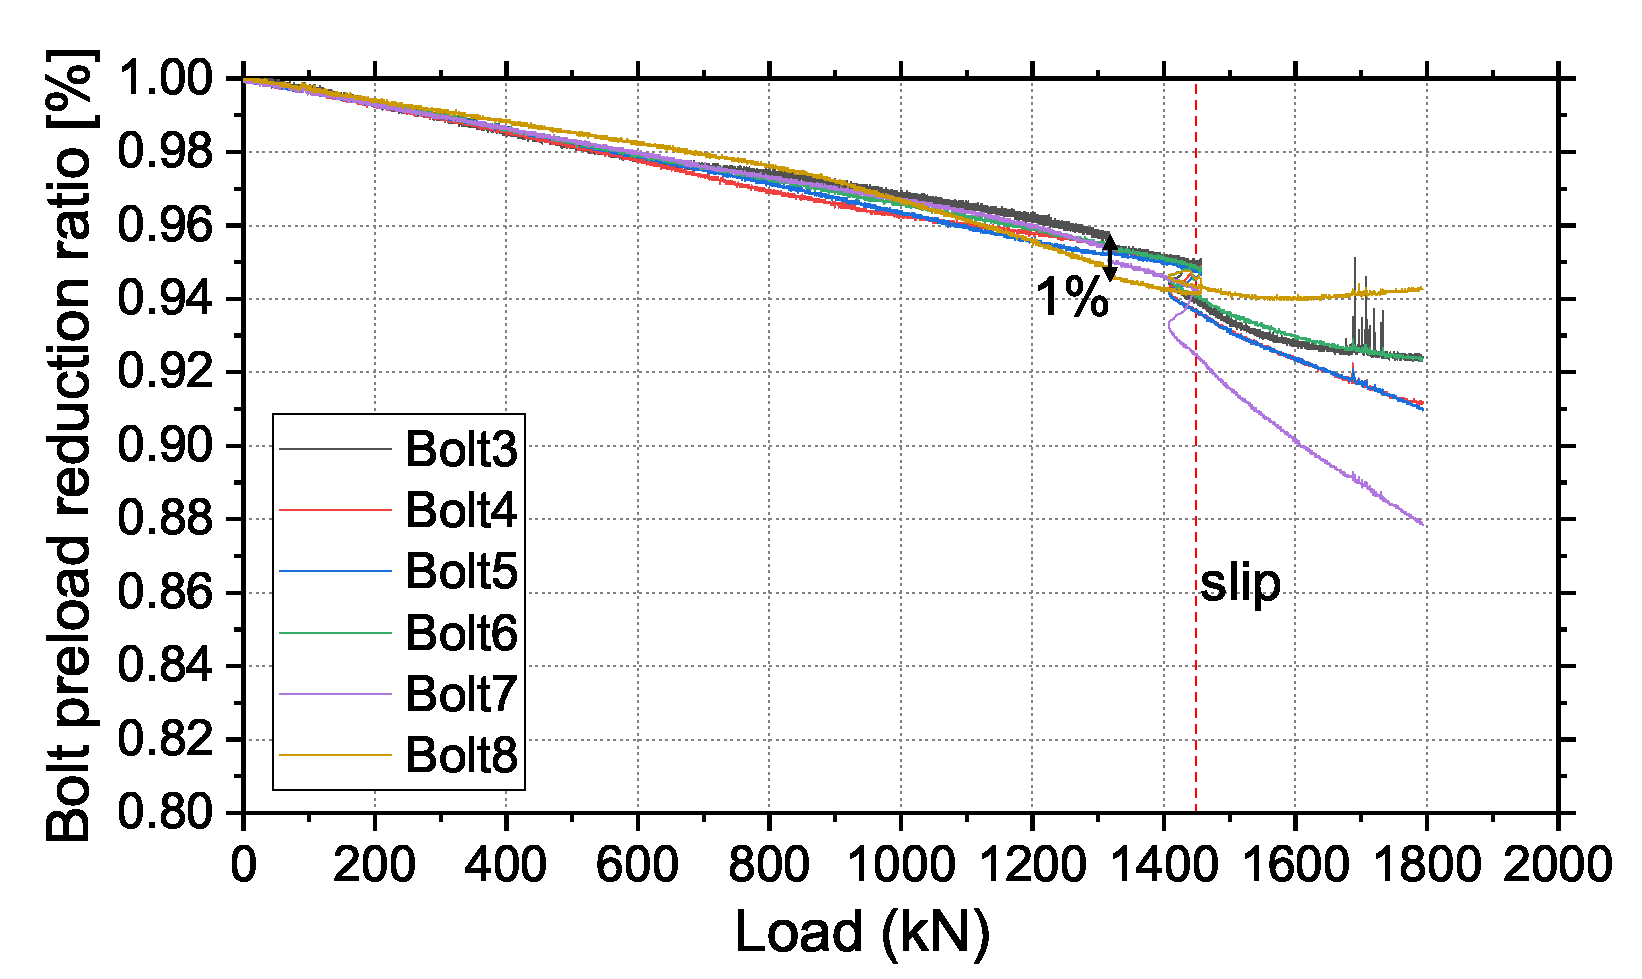
\includegraphics[width=\linewidth]{imgs/ch6/loadaf-hyb.eps}
    \caption{Hybrid joint }
    \label{fig-lafhy}
    \end{subfigure}
    \caption{The relationship between Bolt preload reduction ratio and load of each bolt. [\%]}
    \label{fig-laf}
\end{figure}

\subsection{Distribution of relative displacement}

The Distribution of relative displacement (When load = 0.8$F_{sf}$ = 1088kN, while $F_{sf}$ is Friction type joint slip load) is as shown in Fig. \ref{fig-rdbar}. Green bar represents the friction joint and the orange bar represents the hybrid joint. For the positions RD-1 and RD-2 at the ends of the joint, the relative displacement of the hybrid joint is significantly lower in comparison to the friction type joint. This low relative displacement can be attributed to the interference fit of the bolts \# 1 and \# 2, making it more difficult to generate relative displacement when the elastic slip stage is nearing its end. However, at the other end of the hybrid joint, at interference fit bolts \# 9 and \# 10, the relative displacement at RD8, 9 and 10 is actually higher than that of the friction type joint.It is speculated that the higher relative displacement observed at bolts \#9 and \#10 may be attributed to a suboptimal interference fit.

In addition, the hybrid joint has a more uniform distribution of relative displacement compared to the friction joint. This finding is consistent with the results discussed in section 3.3 regarding the distribution of bolt preload reduction. As a result, it can be inferred that the hybrid joint demonstrates a more uniform load distribution mechanism. The load sharing mechanism discussed in this paper is also similar to the analytical discussions found in previous studies \cite{Chen2023MechanicalConnections}.

\begin{figure}[htbp]
    \centering
    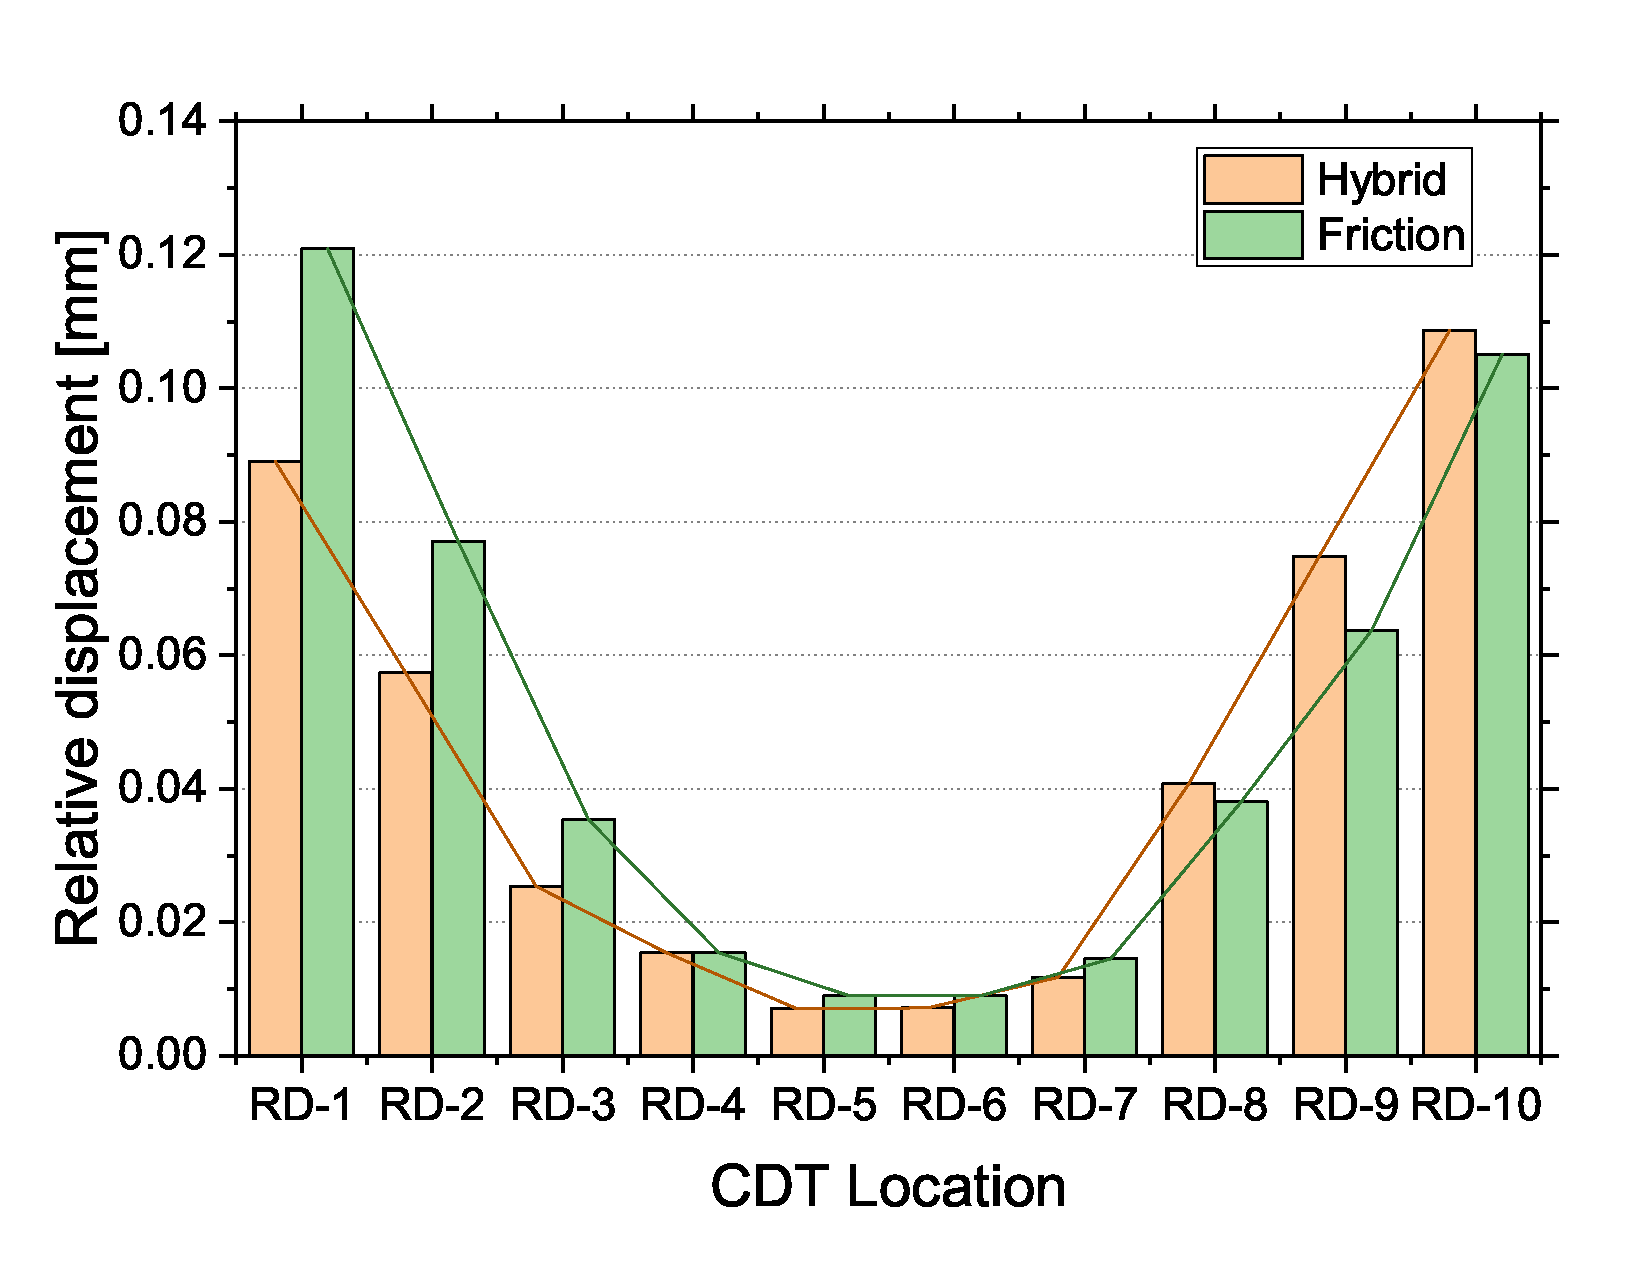
\includegraphics[width=0.6\textwidth]{imgs/ch6/RD-bar.eps}
    \caption{Distribution of Relative displacement (When load = 0.8$F_{sf}$ = 1088kN, while $F_{sf}$ is Friction type joint slip load) }
    \label{fig-rdbar}
\end{figure}

\subsection{Strain of the plate}

The Relationship between Load and strain are shown in Fig. \ref{fig-LS}, Where the measurement position are shown in Fig. \ref{fig-mealoc}. Fig. \ref{fig-s1ss2} shows the S1 and SS2 strain of the end of friction type joint, it is evident that the strain SS2 on the inner side of the splice plate has a steeper slope than S1 of the main plate. This indicates that the inner side of the splice plate undergoes a greater deformation in the tensile direction (referred to as the y-direction) compared to the main plate under the same load. Consequently, the deformation ($0.3\delta_y$) of the splice plate perpendicular to the tensile direction (x-direction) also increases. The deformation of the splice plate in the x-direction (i.e. the reduction in thickness) directly leads to a decrease in the bolt preload. This is because the deformation of the main plate at S1 is suppressed and part of the load is transferred to the splice plate by interfacial friction, causing the deformation of the splice plate at SS2 to be slightly greater than that of the main plate at S1. This also explains why the bolt preload decreased faster for the inner bolt \# 10 than for the outer bolt \# 1.

Compared to the friction joint, the hybrid joint exhibited higher slope of direct strain S1 and load. At 1456 kN, there was a minor slip, resulting in a slight change in slope. However, the strain remained quasi-linear until reaching the maximum load of 1800 kN. In contrast, for the friction joint, non-linear behavior was observed at around 800 kN, possibly due to uneven load distribution, reaching the limit of the end bolts' slip resistance. Due to the reduction in bolt preload, the slip resistance capacity decreases as the load increases until slip occurs.

Furthermore, focus on direct strain at position S3 that has already transmitted a portion of the load through bolt \# 1; this non-linear behavior becomes more evident and there is some residual strain after unloading. Nevertheless, there is no discernible non-linear behavior in the hybrid joint. The slop decreases only slightly during slip and after unloading, remains linear without the presence of residual strain. It can be inferred that the load-strain relationship of the hybrid joint is quasi-linear overall (up to the maximum load of 1800kN).

\begin{figure}[htbp]
\centering
    \begin{subfigure}[t]{0.6\textwidth}
        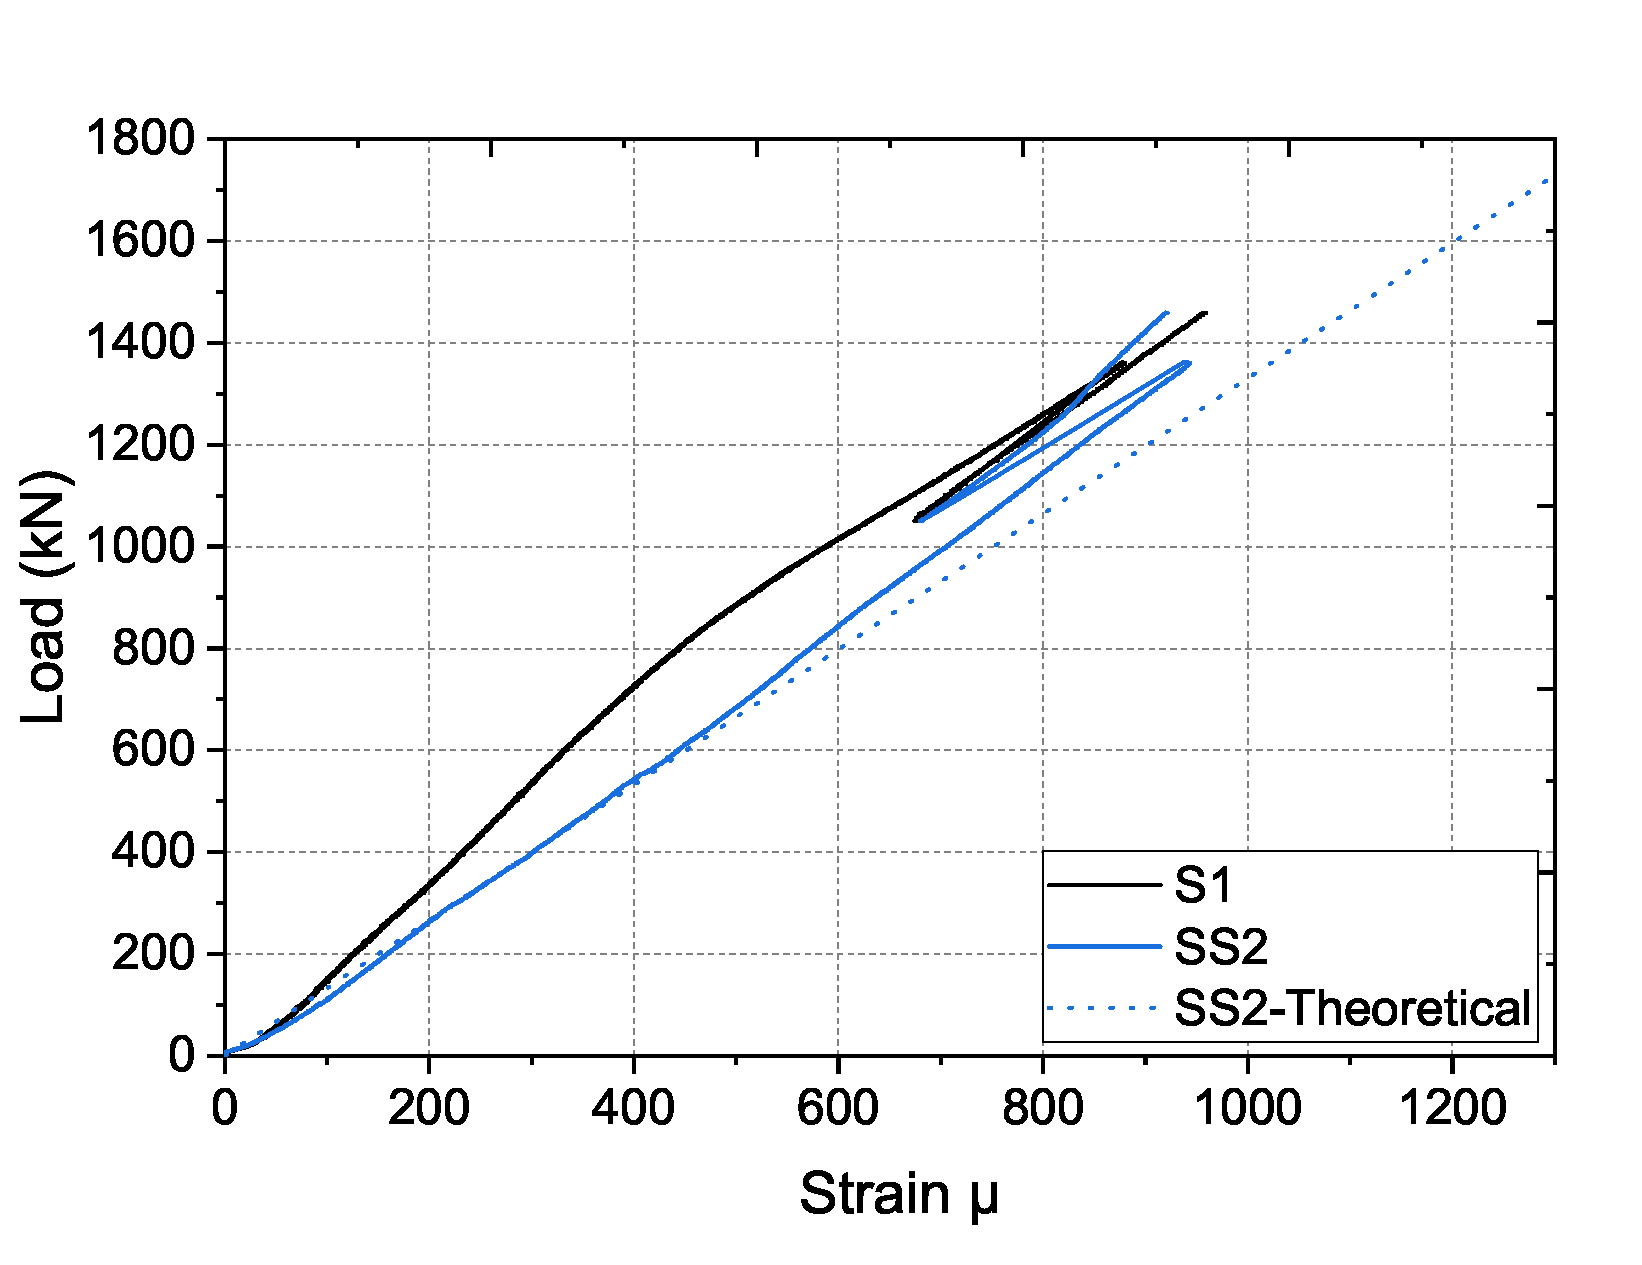
\includegraphics[width=\linewidth]{imgs/ch6/S1SS2-F.eps}
        \caption{S1,and SS2 for Friction type joint}
        \label{fig-s1ss2}
    \end{subfigure}
    \hfill
    \begin{subfigure}[t]{0.6\textwidth}
        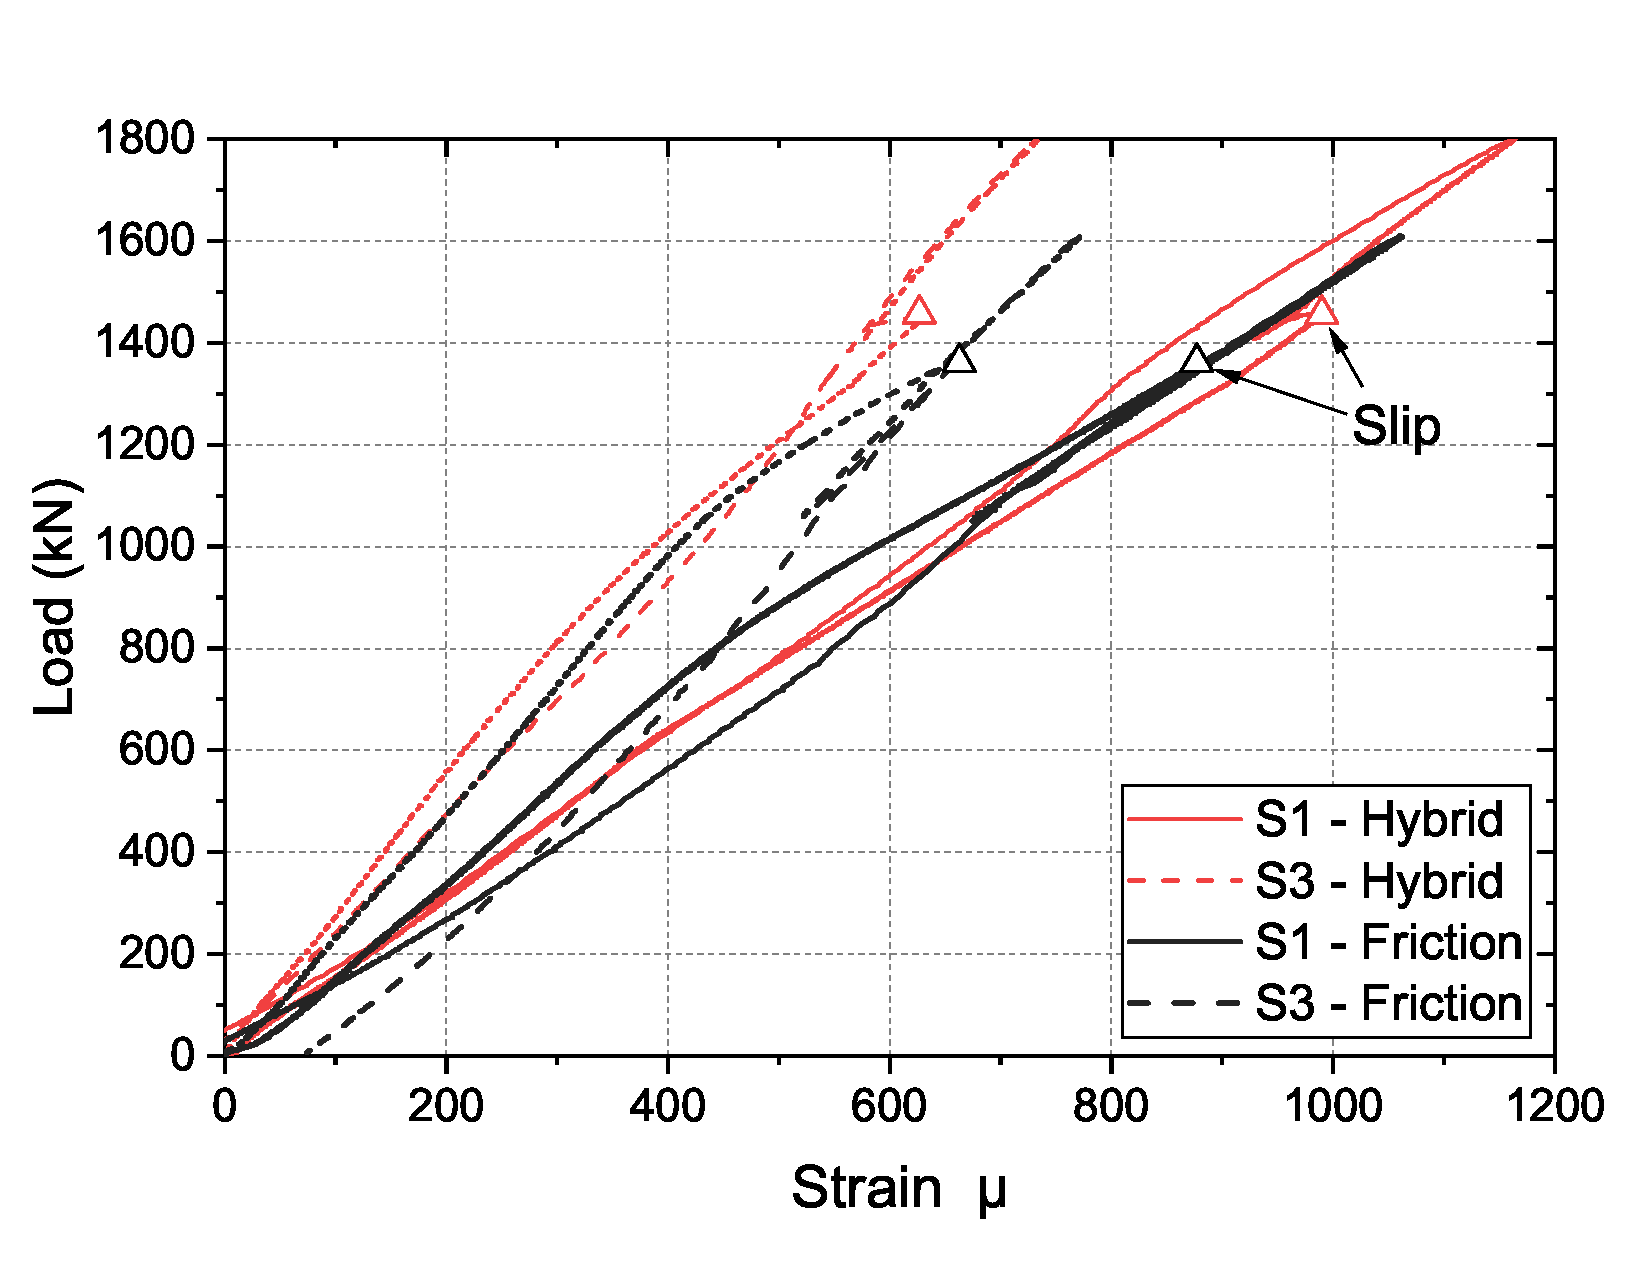
\includegraphics[width=\linewidth]{imgs/ch6/S3-FH.eps}
        \caption{s1 and s3 for Friction and Hybrid joint}
        \label{fig-s3FH}
    \end{subfigure}
    \caption{Relationship between Load and Direct Strain}
    \label{fig-LS}
\end{figure}

\section{Discussion}

\subsection{Cross-section observation after slipping}

Fig. \ref{fig-csob} shows the Cross-section of Hybrid joint. The cross-sectional diagram was obtained from the hybrid joint that underwent a load of up to 1800kN. Fig. \ref{fig-csob1} shows the cross-sectional diagram of bolts \#1 - \# 3, revealing that the deformation of the rib on the non-bearing side is very small as observed in the magnified portion of bolt \#1 on the right side. Likewise, the magnified section of Bolt \#2 on the opposite side of the bearing suggests minor deformation of the rib. It appears that some ribs do not make contact with the hole wall when the interference fit bolt is hammered into the hole. Consequently, the desired interference fit is not produced, resulting in a minor slip in the joint. This slip is believed to be caused by the clearance created during the bolt installation, as well as slight plastic deformation of the rib.

\begin{figure*}
    \centering
    \begin{subfigure}[t]{0.85\textwidth}
    \centering
    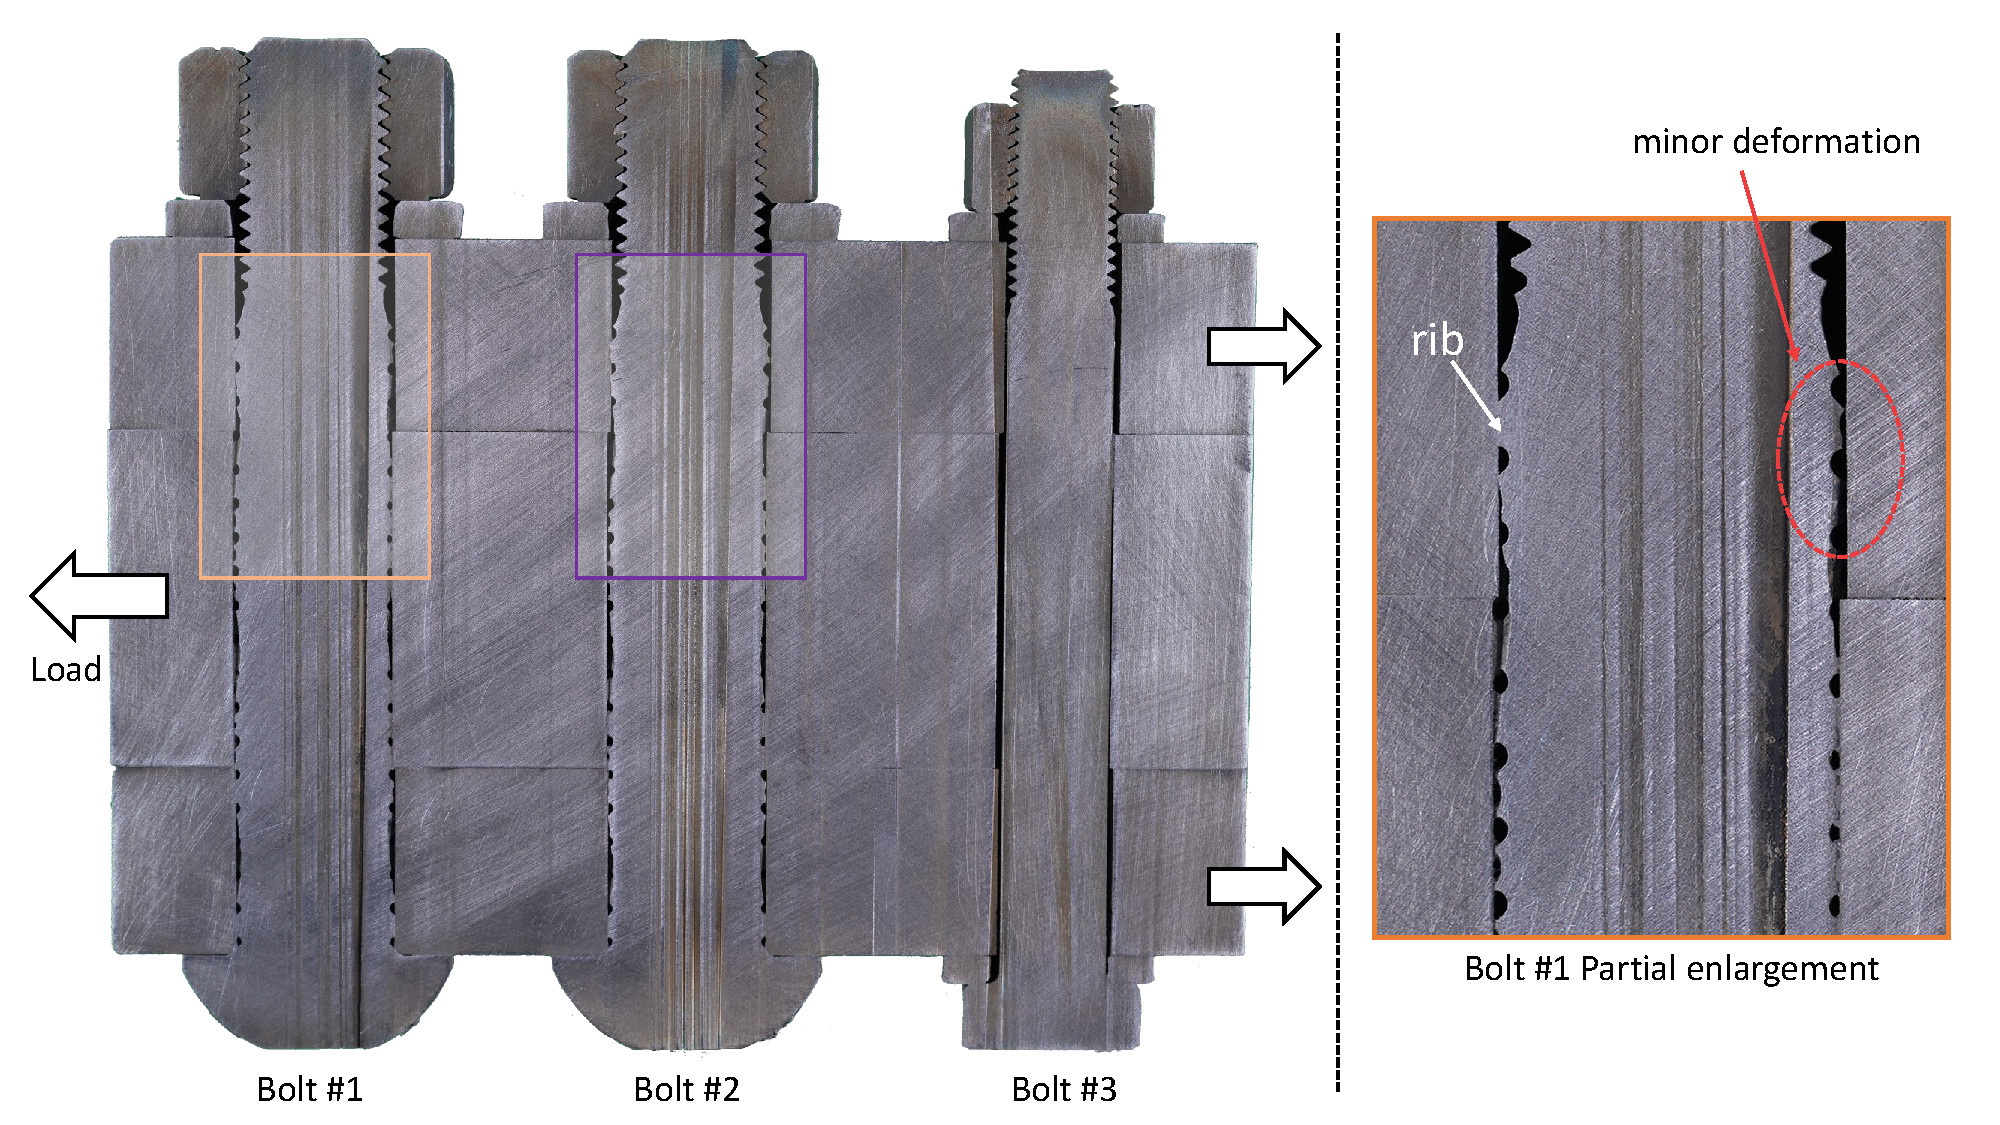
\includegraphics[width=\linewidth]{imgs/ch6/cros-sec-ob1.pdf}
    \caption{Bolt \#1 -- \#3}
    \label{fig-csob1}
    \end{subfigure}
    %\vspace{1cm}
    \begin{subfigure}[t]{0.85\textwidth}
    \centering
    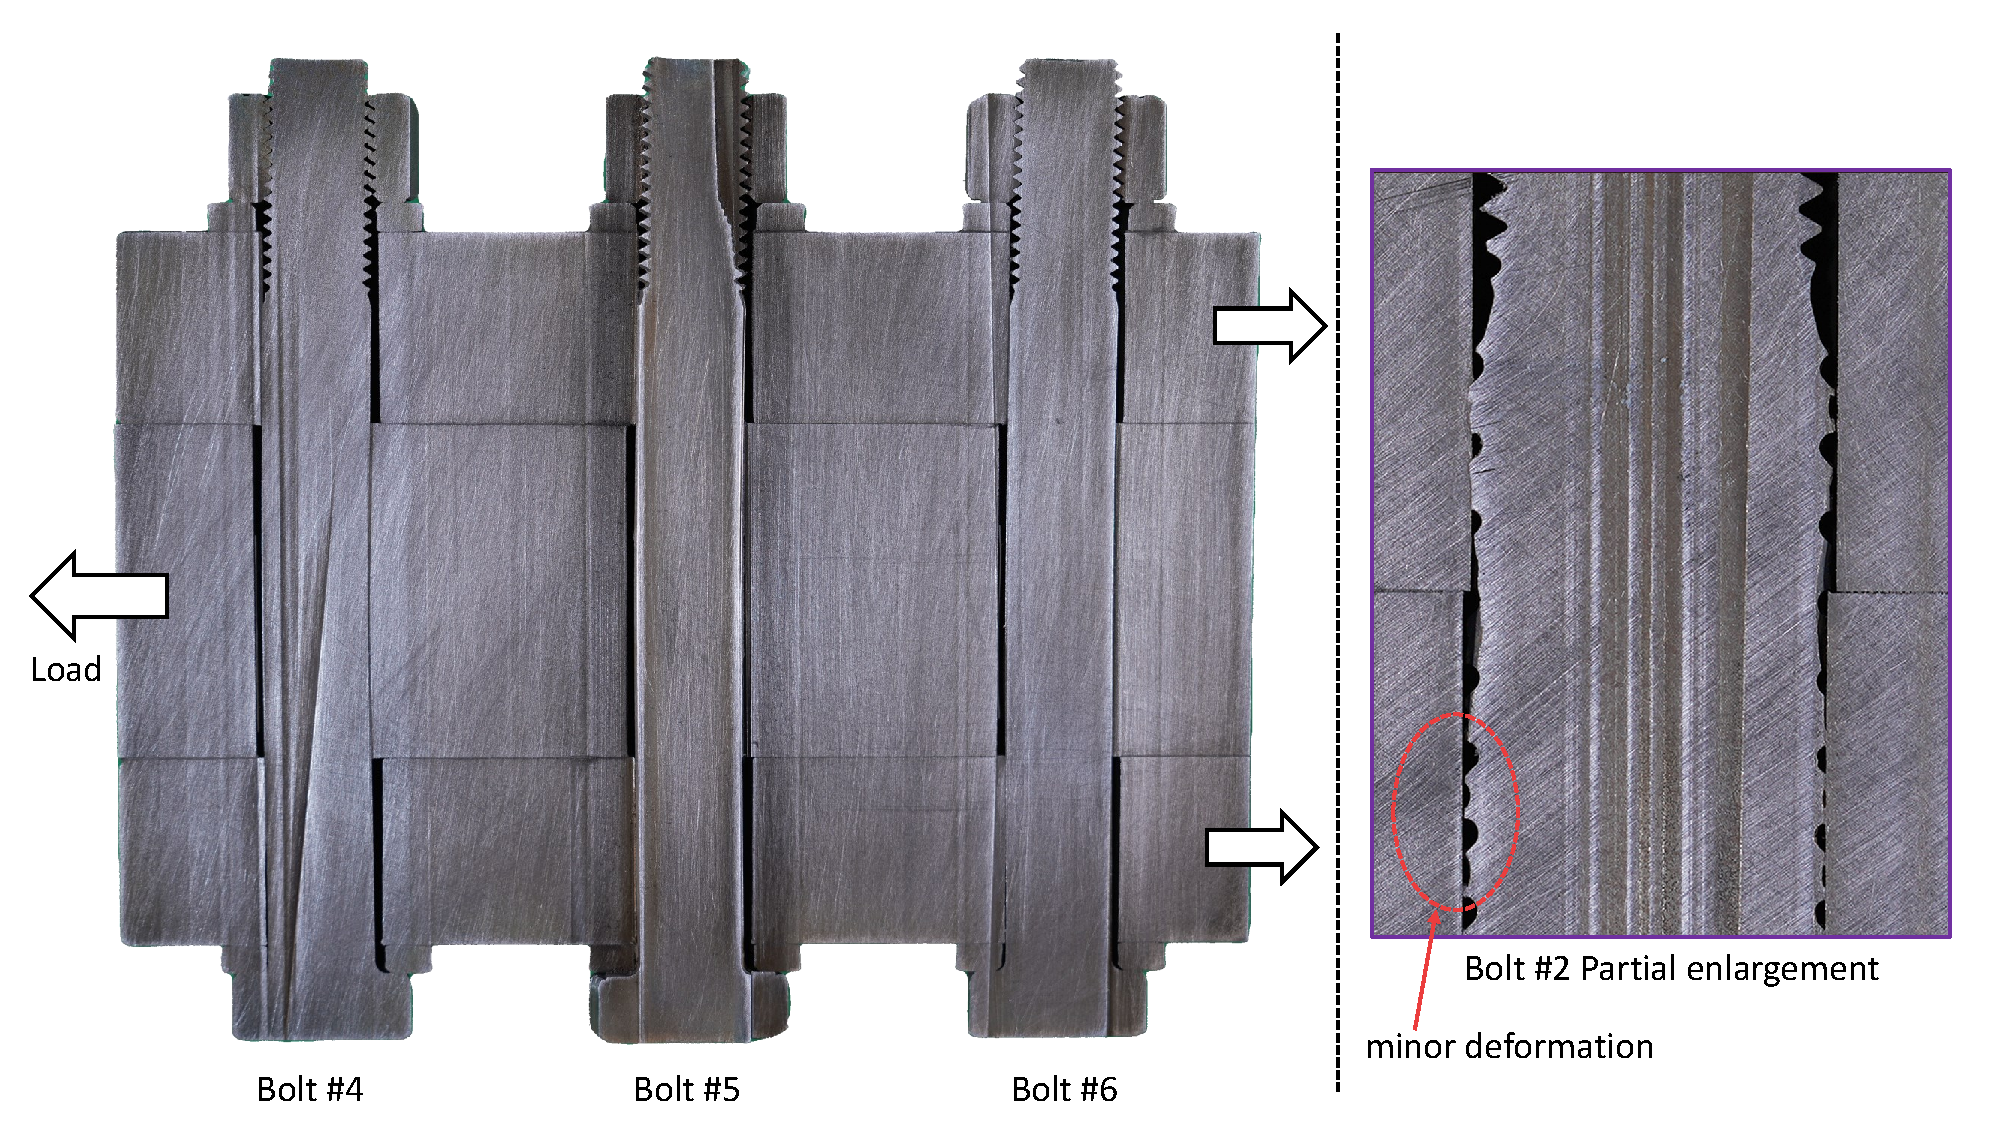
\includegraphics[width=\linewidth]{imgs/ch6/cros-sec-ob2.pdf}
    \caption{Bolt \#4 -- \#6}
    \label{fig-csob2}
    \end{subfigure}
    \caption{Cross-section of Hybrid joint's each bolt, Loading to 1800kN}
    \label{fig-csob}
\end{figure*}


Fig. \ref{fig-dicdisp} shows the displacement of the hybrid joint case at a load of 200kN, measured by DIC methods, taken from the side of the joint. It was found that the displacement on the nut side of the joint (i.e. SP2 side) is greater than the displacement on the bolt head side (i.e. SP1 side). This observation is consistent with the results obtained from cross-sectional observations. Insufficient interference fit resulted in an increase in displacement and a slight occurrence of slippage.

\begin{figure*}
    \centering
    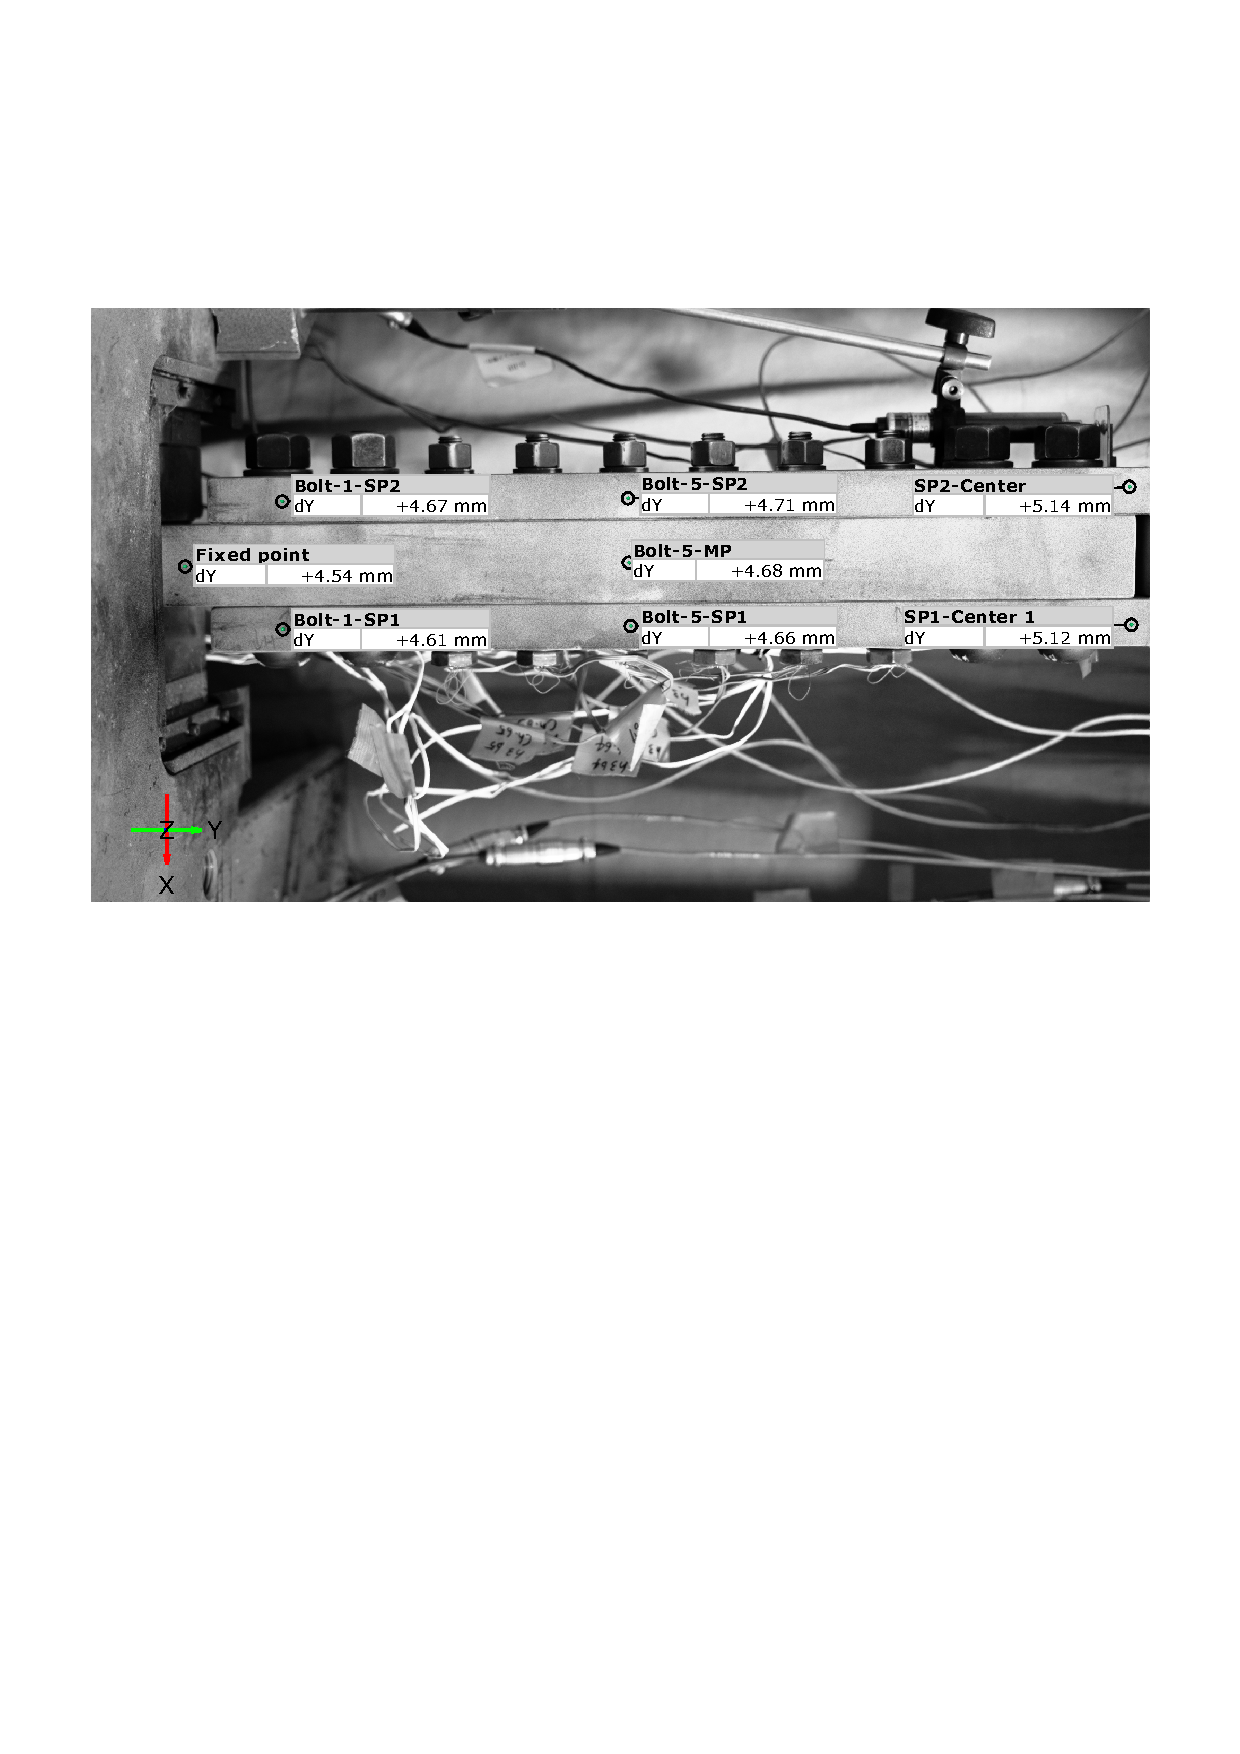
\includegraphics[width=0.85\linewidth]{imgs/ch6/dic-B3-200kN.pdf}
    \caption{Displacements of hybrid joint when load is 200kN }
    \label{fig-dicdisp}
\end{figure*}

\subsection{Load reduction for long bolted joint}

The European Convention for Constructional Steelwork (ECCS), and ISO/TC specify that the resistance should be reduced by a factor of $\beta_{rd}$ when the spacing between the first and last bolt in a joint is larger than 15d as shown in Eq.\ref{eq-eurolon} \cite{eccs1985,isohtb}. AASHTO \cite{AASHTO2020} provides the nominal shear resistance of bolts in joints longer than 38.0 in. must be reduced by an additional factor of 0.83 or 0.75/0.9\par

\begin{equation}\label{eq-eurolon}
    \beta_{rd} = 
    \begin{cases}
    1 & (L \leq 15 d) \\ 
    1.08-L / (200 d) & (15 d < L \leq 65 d)\\ 
    0.75 & (65 d < L)
    \end{cases}
\end{equation}

Eurocode 3 (EN 1993-1-8:2005) \cite{eurocode3-21} provisions that where the distance $L_j$ between the centers of the end fasteners in a joint, measured in the direction of force transfer is more than 15d, the design shear resistance of all the fasteners should be reduced by multiplying it by a reduction factor $\beta_{Lf}$:
\begin{equation}
    \beta_{Lf}=1-\frac{L_j - 15d}{200d}
\end{equation}

Japanease Specification for Highway Bridge (JSHB) \cite{douji2017} published by Japan Road Association states that when the number of row exceeds 8 in bolted joint, a reduction factor must be applied to the slip resistance, as shown in Table \ref{ch6tab-jpredu}.
\begin{table}[h]
    \centering
    \caption{Reduction of slip resistance of bolted joint of JSHB-JRA}
    \begin{tabular}{cccccc}
    \toprule
        Number of Row &  8 & 9 & 10 & 11 & 12 \\ \midrule
        Reduction factor & 1.00 & 0.98 & 0.96 & 0.94 & 0.92 \\ \bottomrule
    \end{tabular}
    \label{ch6tab-jpredu}
\end{table}

Furthermore, due to the non-uniformity of load distribution, the bolts are unable to fracture simultaneously, consequently leading to a reduction in the ultimate limit bearing capacity.\cite{Takai2021BoltUnbuttoning,Peng2013FeaDimensions,peng2010}.

Table \ref{tab-rera} presents the experimentally acquired slip loads $P_{s}$ of each case, along with their corresponding calculated slip resistance $F_{ds}$. It also shows the load reduction rate between the experimentally acquired slip loads $P_{s}$ and the calculated values $F_{ds}$. Eurocode 3 \cite{eurocode3-21} recommend that interference fit bolts should be designed by calculating slip resistance in the same way as HSB friction type connection. Slip resistance $F_{ds}$ is calculated from Equation \ref{eq-fds1ch6} and slip load $P_s$ is the load when the first load drop occurred. The lengths of the Friction and Hybrid joint $L_j$ are both 495 mm (where $L_j$ is the distance between the centres of the end fasteners in a joint). The load reduction rate of the friction type reaches 0.79, which is lower than the values specified by Eurocode (calculated to be 0.92) and JHSB (calculated to be 0.96). It is inferred that this is due to the use of thick plate (50mm in main plate) in this experiment. Because the thick plate causes the bearing stress on the bolt to be uneven, the bolt will be more susceptible to bending deformation, resulting in loss of preload. While the Hybrid joints have a slip load reduction of 0.9, which is about 10\% higher than friction joints. The slip resistance reduction ratio for the hybrid joint without preload (Hybrid-NAF case) on the interference fit bolts was 0.92, which is approximately the same as for the hybrid joint. This is because regardless of the presence of preload in the interference fit bolt, the amount of slip until the load is increased is nearly the same for both cases. This depends on the gap in the bolt and hole wall and the plastic deformation of the rib. 



\begin{table}[]
\centering
\caption{Slip resistance reduction ratio of each case}
\begin{tabular}{@{}lccc@{}}
\toprule
 & \begin{tabular}[c]{@{}c@{}}Slip load $P_s$\\ kN\end{tabular} & \begin{tabular}[c]{@{}c@{}}slip resistance $F_{ds}$\\ kN\end{tabular} & load reduction rate \\ \midrule
Hybrid & 1456 & 1618 & 0.90 \\
Hybrid-NAF & 1237 & 1341 & 0.91 \\
Friction & 1362 & 1726 & 0.79 \\ \bottomrule
\end{tabular}
\label{tab-rera}
\end{table}

\begin{equation}
    \label{eq-fds1ch6}
    F_{ds} = \sum_n \mu \times N_0 \times m
\end{equation}

where $\mu$ is the slip coefficient = 0.8 taken from the slip factor test which arranged two bolts and has the same plate thickness and the same faying surface condition as this test, $N_0$ is the preload of the bolts before loading, $m$ is the number of shear planes, $n$ is the number of the bolt.


In addition, the theoretical calculations indicate that applying a preload of 106kN to a bolt with a diameter of 22mm would result in a contraction of 0.009 mm, which is much smaller than the manufacturing tolerances of the bolt hole or the bolt shank diameter. Therefore, the horizontal shrinkage of the bolt shaft is small enough to be negligible.

Bolt shaft shrinking value ($\Delta d$) is:
\begin{equation}
    \label{eq-bdefo}
    \Delta d=\delta_{yb}d_{ib}=\frac{N_0v}{EA}d
\end{equation}
where $\delta_{yb}$ is the bolt strain of y-direction (axial direction), $d_{ib}$ is the diameter of the interference fit bolt, $A_{ib}$ is the cross-sectional area of the interference fit bolt shaft.

Therefore, result as the amount of bolt preload does not have a significant effect on the slip behavior, and it can be considered that the reduction of slip load is related to the bearing capacity of the rib, as insufficient contact area of the rib results in excessive contact pressure and compression plastic deformation. 

\begin{figure}[htbp]
    \centering
    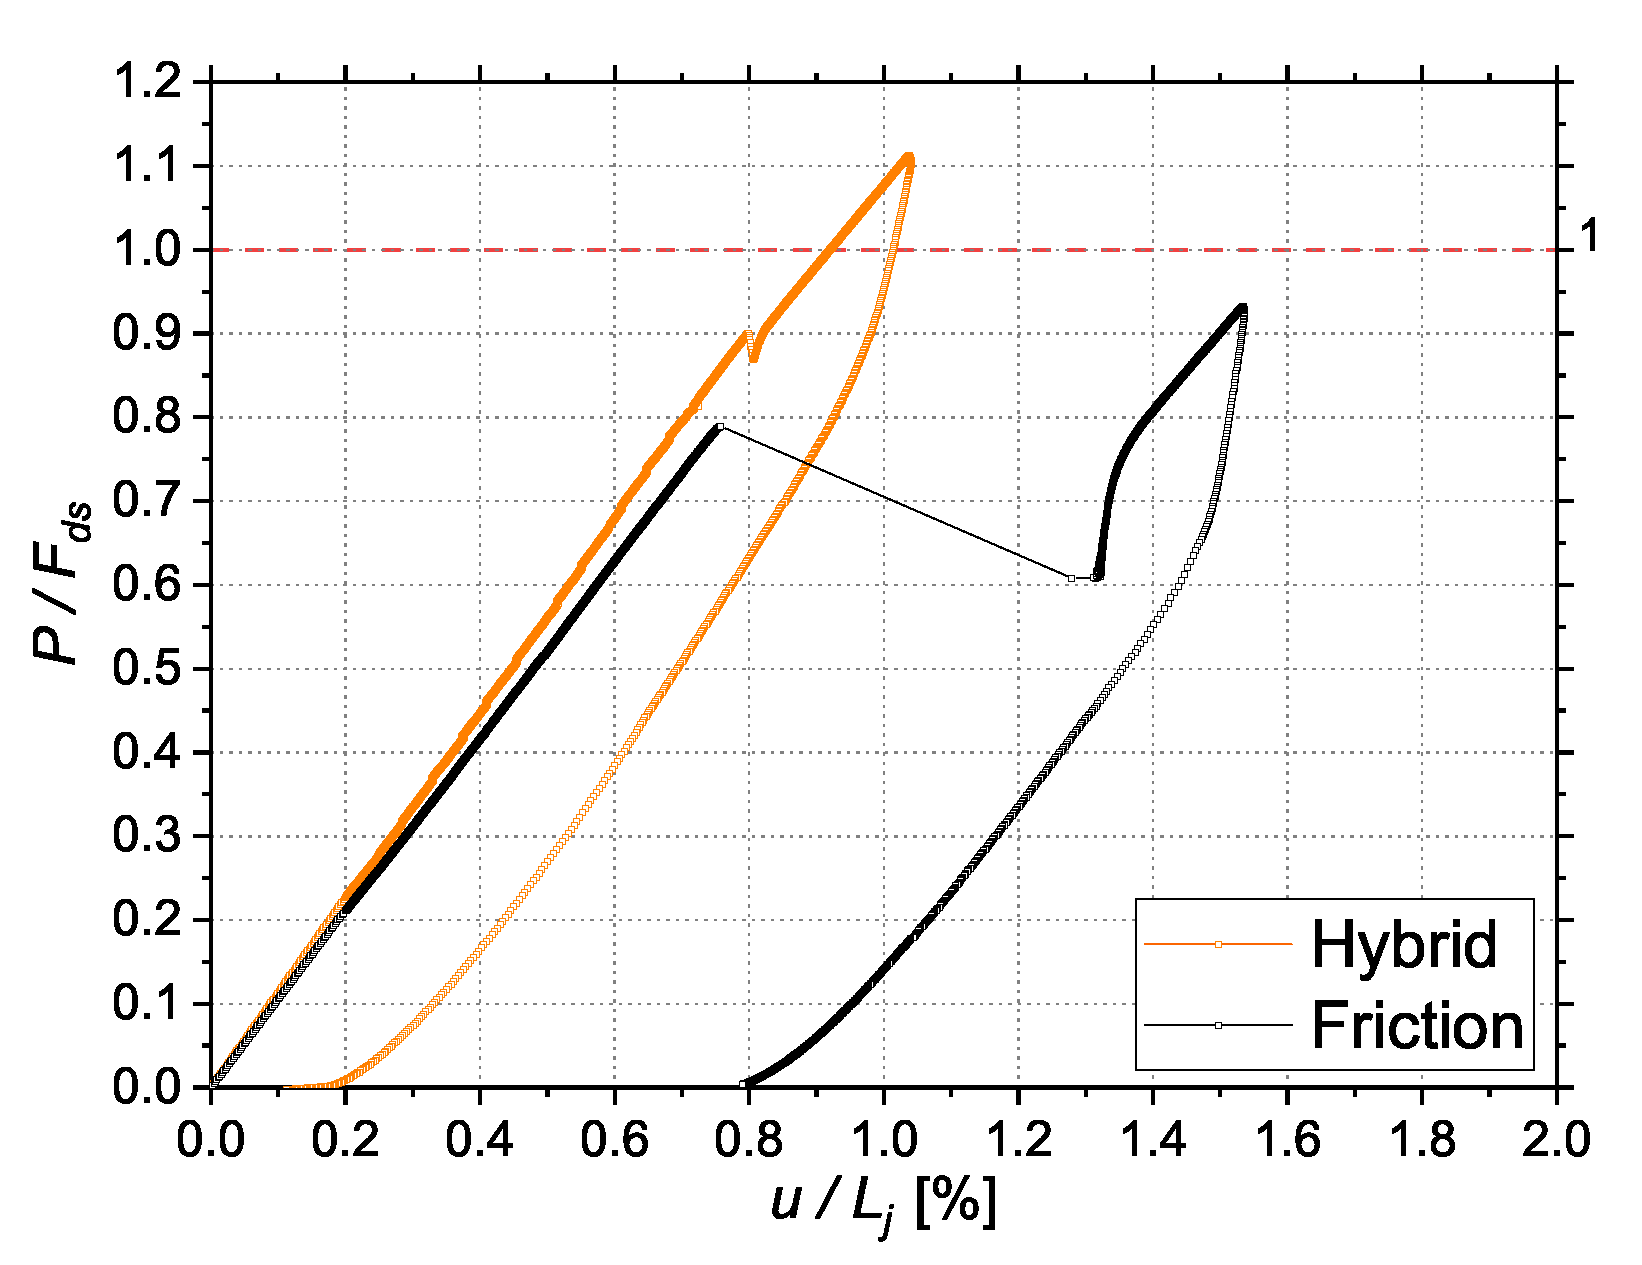
\includegraphics[width=0.6\textwidth]{imgs/ch6/nor-load-disp.eps}
    \caption{The relationship between normalised load and normalised deformation. (Normalised load is the load divided by the sliding load $F_s$, and normalised deformation is the deformation divided by the joint length $L_j$).}
    \label{fig-ldnor}
\end{figure}

Fig. \ref{fig-ldnor} shows the relationship between normalised load and normalised deformation. It can be seen that the initial slop is higher for the Hybrid-NAF case, this is due to the bearing resistance of the interference fit bolts is not included in the calculation of the slip resistance, comparing this with the behaviour of the friction joint, it can be confirmed that the bearing resistance is included in the load sharing of the Hybrid-NAF joint result a high initial slope of Hybrid-NAF case, despite the minor amount of slip that occurs. The minor amount of slip is due to the inadequacy of the interference fit,  which results in the interference fit bolt in not being able to fully resist the portion of the load lost as a result of the slip that occurs. 


\subsection{Limit state}

Previous study \cite{fisher1965behavior} shows that load will firstly transmit by the connection with higher stiffness, and the bearing-type connection will only play a significant role in load sharing when the friction-type connection approaches its limit. Therefore, the limit state of a hybrid joint relies on the state of the bearing type connection, which can manifest as either the shear yield limit of the bolt or the bearing deformation limit of the main plate.

This study considers that for hybrid joints using bearing type bolted connections and friction connections together, the design under the serviceability limit state can be performed by accumulating the bearing resistance of interference fit bolt and the slip resistance of HSB.

However, in this experiment, slight slippage occurred in the hybrid joint, which was believed to be caused by the gaps between the rib and the hole wall. Therefore, regarding the definition of the limit state of the hybrid joint, by referring to the Japanese AIJ Recommendations for Design of Connections in Steel Structures \cite{2012AIJStructures}, a slip limit of 0.2mm can be set for the joint. The maximum load within a relative slip coefficient of 0.2mm is taken as the serviceability limit state, which is the slip resistance $F_{ds}$ in Table \ref{tab-rera}. Since a slight slip occurred in the hybrid joint in this experiment, the behavior after 0.2 mm cannot be determined based on this data. 

Despite this, hybrid joints in the slip limit state exhibit greater strength compared to friction joints. The load distribution is also more even and the relative displacement of the ends is smaller. Consequently, the performance of hybrid joints is superior to that of existing friction joints under the current slip limit specification, and the study concludes that designing hybrid joints under the current slip limit specification is feasible.

\section{Summarize}

This study focuses on interference fit bolts assembled at both ends of friction type bolted joint to elucidate the slip resistance and deformation of the hybrid joints, and to verify whether the interference fit bolts can be assembled in the friction type joints to improve the strength of the joint. Tensile tests were performed with three specimens: friction type bolted joint, hybrid joint, and hybrid joint with non-preload interference fit bolts. 

On the basis of the results of our investigation, we have made the following findings and conclusions. \par

\begin{enumerate}

\item The slip load of a 10-row hybrid joint assembled with four interference fit bolts at both ends is approximately 7\% higher than that of a friction-type joint. If the initial preload of the bolts is considered inconsistent, the result of dividing the slip load by the corresponding calculated slip resistance is approximately 10\% higher for the hybrid joint than that for the friction-type joint.

\item The distributions of relative displacements and reduction in the preload on the individual bolts of the joint show that the hybrid joint has a small dispersion of the data when compared with the friction-type joint, suggesting that the uneven load distribution and deformation of the joint can be improved by installing interference fit bolts. This allows the inner bolts of the hybrid joint to share a greater part of the load than the friction-type joint for the same load level, thus reducing the load concentration on the outer bolts. The deformation of the hybrid joint improves owing to the considerable reduction in the outermost relative displacement RD1. The performance of hybrid joints is superior to that of the existing friction-type joints under the current slip limit specification. 

\item The overall load--deformation relationship of the hybrid joint remains quasi-linear up to the upper load limit of 1800 kN, although a minor amount of slip occurs. Moreover, the total residual deformation of the hybrid joint is only 0.2\% relative to the length $L_j$ of the joint. In contrast, the friction-type bolted joint produces a residual deformation of 0.75\% when loaded to 1600 kN. Therefore, within the quasi-linear range, it can be expected that the hybrid joint will have a high serviceability limit strength.

\item The observation of the cross section showed that the rib portion of the interference fit bolt tail did not provide a good interference fit (the rib was not in contact with the hole wall or the contact area was too small). This resulted in the interference fit bolt being unable to fully resist the portion of load lost due to the slip, causing a minor slip to occur. This is also illustrated by the fact that the displacement of the splice plate SP2 on the nut side is greater than that of the splice plate SP1 on the head side of the bolt.


\end{enumerate}